\documentclass[11pt,a4paper,onecolumn]{article}
\usepackage[T1]{fontenc}
\usepackage[utf8]{inputenc}
\usepackage{lmodern,microtype}
\usepackage[margin=1in]{geometry}
\usepackage{amsmath,amssymb,amsthm,mathtools}
\usepackage{booktabs,tabularx,array,enumitem,float,needspace}
\usepackage[section]{placeins}
\usepackage{tikz}
\usetikzlibrary{arrows.meta,positioning,fit,calc}
\usepackage[framemethod=default]{mdframed}
\usepackage{xcolor}
\usepackage[hidelinks]{hyperref}
\usepackage[nameinlink,noabbrev]{cleveref}
\usepackage{fancyhdr}
\hypersetup{pdftitle={An Authenticated Live Sequencer Stream},
pdfsubject={Regional SMR, status-aware cross-region rotation, and rollup derivation}}
\setlength{\headheight}{14pt}
\pagestyle{fancy}\fancyhf{}
\lhead{\small An authenticated live sequencer stream}\rhead{\small Version 4 / discussion draft}
\cfoot{\thepage}
\setlength{\emergencystretch}{2em}
\setlist{nosep,leftmargin=*}
\newcolumntype{Y}{>{\raggedright\arraybackslash}X}
\newcommand{\Hash}{\mathsf H}
\newcommand{\Sig}{\mathsf{Sign}}
\newcommand{\QC}{\mathsf{QC}}
\newcommand{\gv}{v_{\mathrm G}}
\newcommand{\lv}{v_{\mathrm L}}
\newcommand{\pre}{\preceq}
\newcommand{\wt}{\operatorname{wt}}
\newcommand{\rank}{\operatorname{rank}}
\newcommand{\Tag}[1]{\ensuremath{\mathsf{#1}}}
\newcommand{\Proc}[1]{\textnormal{\textsc{#1}}}
\newtheorem{definition}{Definition}[section]
\newtheorem{assumption}[definition]{Assumption}
\newtheorem{lemma}[definition]{Lemma}
\newtheorem{theorem}[definition]{Theorem}
\newcounter{protocol}
\newenvironment{protocol}[2]{\refstepcounter{protocol}\label{#1}
\begin{mdframed}[nobreak=true,linewidth=.6pt,skipabove=9pt,skipbelow=9pt,
innertopmargin=7pt,innerbottommargin=7pt]\small
\noindent\textbf{Protocol \theprotocol. #2}\par\smallskip}{\end{mdframed}}
\crefname{protocol}{Protocol}{Protocols}
\Crefname{protocol}{Protocol}{Protocols}
\crefname{definition}{Definition}{Definitions}
\crefname{assumption}{Assumption}{Assumptions}
\crefname{lemma}{Lemma}{Lemmas}
\crefname{theorem}{Theorem}{Theorems}
\title{An Authenticated Live Sequencer Stream\\
\large Regional SMR and Status-Aware Cross-Region Rotation}
\author{}\date{29 September 2026}
\begin{document}
\maketitle
\begin{abstract}
We specify an authenticated mini-block stream across regional sequencing
groups. A cross-region service composes regional live-stream interfaces:
a new group starts only after verifying its predecessor's finalized anchor.
Regular rotation follows a fixed batch quota and a predefined region list,
skipping unavailable regions. A regional status committee authenticates only
an entry consisting of a future L1 activation height and a region-status
map. Each mini-block header binds a finalized L1 height as its logical
timestamp. An announced update takes effect only at its scheduled control
height, after a preparation window; it forces a handoff only if the region
authorized at that boundary becomes unavailable. Recovery of an inactive
region changes future eligibility. We instantiate
the regional service with Sync HotStuff, define cross-region control and
rollup-derivation relations, and separate four operating paths in the latency,
throughput and communication analysis. Forced recovery preserves final
prefixes under an explicit closed-cut and data-recovery assumption.
\end{abstract}

\noindent\textbf{Version 4 scope.}
This version preserves the inherited specification and adds
\cref{sec:rotation-discussion} on normal local leader rotation and production
HotStuff-family designs. The tentative quota-triggered BLAME condition in
step V1 remains an experiment: the regional progress proof below covers the
original missing-progress/equivocation triggers, not that added condition.
The new handoff and pipeline alternatives are discussion proposals, not
additional established guarantees.

\section{Architecture and Service Goals}\label{sec:architecture}
A region is a group of sequencers that orders batches of mini-blocks using
state machine replication (SMR). A mini-block contains an ordered transaction
list and an authenticated header. Proposer $P$ consumes this stream, verifies
it, executes its transactions, and publishes data and state commitments.
Sequencers may execute privately to choose an order; the sequencing service
itself certifies ordering. The layer-one blockchain (L1) supplies finalized
configuration and control records, while a data-availability (DA) mechanism
supports retrieval of the published data.

The cross-region service coordinates successive regional streams. A
\emph{session} is one region's authorized production instance, and an
\emph{anchor} is the finalized stream checkpoint from which it starts.
The cross-region service, called the \emph{wrapper} below, opens a session,
consumes its confirmed outputs, and transfers authority at a verified
boundary. Regions
do not run an additional crash-fault-tolerant consensus protocol over each
other's state transitions. Regional safety, committee-entry integrity and
L1 finality have separate assumptions.

A \emph{term} is one region's production turn, with a configured quota
of $K\geq1$ application batches. There are three distinct transitions:
\begin{itemize}
\item A \emph{local view change} replaces the leader inside the same region
and preserves the current term and its remaining quota.
\item A \emph{regular cross-region rotation} transfers authority after
the term's $K$ application batches have been finalized.
\item A \emph{forced cross-region rotation} responds when a previously
announced status update becomes effective and makes the then-authorized
region unavailable.
\end{itemize}
Both cross-region paths use the installed cyclic list and skip unavailable
regions. Announcement alone changes no authority. An effective status
change at an inactive region does not interrupt the current term.

\begin{figure}[htbp]\centering
% Native manuscript-sized TikZ. No outer SMR or committee stream attestation.
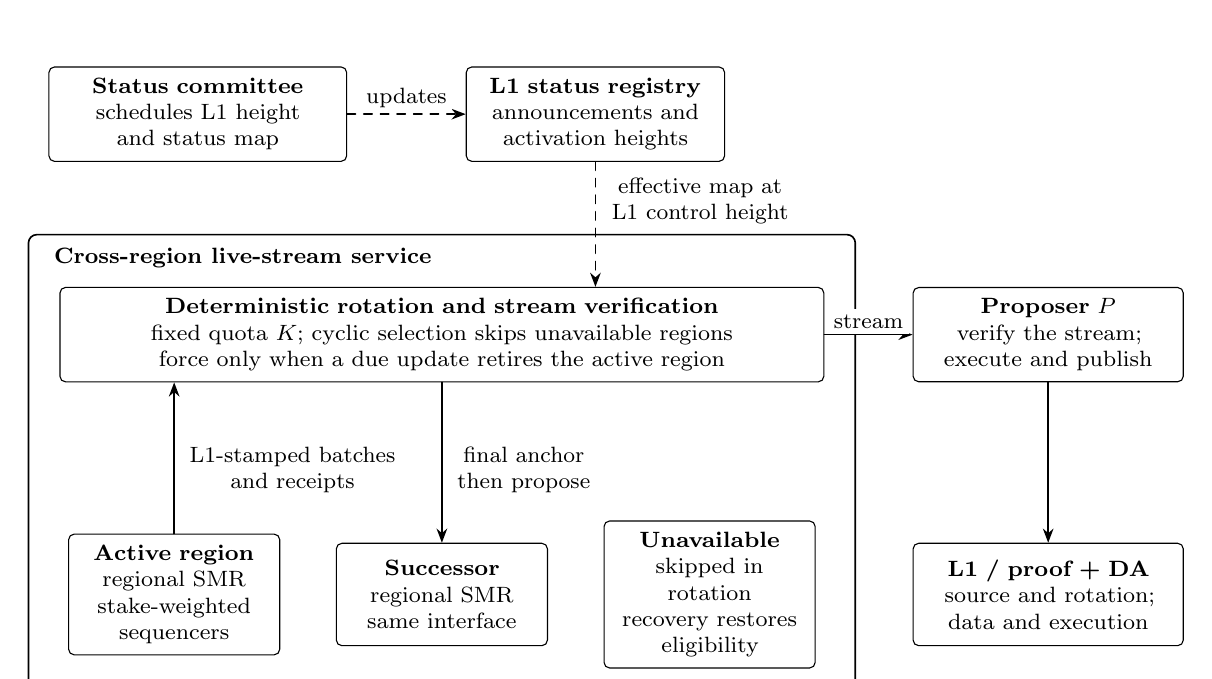
\begin{tikzpicture}[
  x=1cm,y=1cm,font=\footnotesize,line cap=round,line join=round,
  box/.style={draw,rounded corners=2pt,fill=white,align=center,
    inner sep=4pt,minimum height=.72cm},
  flow/.style={-{Stealth[length=1.8mm]},semithick},
  ctl/.style={flow,dashed},
  lab/.style={fill=white,inner sep=2pt,align=center}
]
  \node[box,text width=3.5cm] (committee) at (2.3,7.25)
    {\textbf{Status committee}\\schedules L1 height and status map};
  \node[box,text width=3.0cm] (registry) at (7.35,7.25)
    {\textbf{L1 status registry}\\announcements and activation heights};
  \draw[ctl] (committee.east) -- node[lab,above] {updates} (registry.west);

  \draw[rounded corners=3pt,semithick] (.15,-.05) rectangle (10.65,5.72);
  \node[anchor=west,font=\footnotesize\bfseries] at (.35,5.43)
    {Cross-region live-stream service};
  \node[box,text width=9.42cm,minimum height=1.1cm] (wrapper) at (5.4,4.45)
    {\textbf{Deterministic rotation and stream verification}\\
    fixed quota $K$; cyclic selection skips unavailable regions\\
    force only when a due update retires the active region};
  \draw[ctl] (registry.south) -- (registry.south |- wrapper.north);
  \node[lab,anchor=west] at (7.48,6.15) {effective map at\\L1 control height};

  \node[box,text width=2.4cm,minimum height=1.3cm] (active) at (2.0,1.15)
    {\textbf{Active region}\\regional SMR\\stake-weighted sequencers};
  \node[box,text width=2.4cm,minimum height=1.3cm] (next) at (5.4,1.15)
    {\textbf{Successor}\\regional SMR\\same interface};
  \node[box,text width=2.4cm,minimum height=1.3cm] (offline) at (8.8,1.15)
    {\textbf{Unavailable}\\skipped in rotation\\recovery restores\\eligibility};
  \draw[flow] (active.north) -- (active.north |- wrapper.south);
  \node[lab,anchor=west] at (2.12,2.73) {L1-stamped batches\\and receipts};
  \draw[flow] (next.north |- wrapper.south) -- (next.north);
  \node[lab,anchor=west] at (5.52,2.73) {final anchor\\then propose};

  \node[box,text width=3.15cm,minimum height=1.13cm] (proposer) at (13.1,4.45)
    {\textbf{Proposer $P$}\\verify the stream;\\execute and publish};
  \draw[flow] (wrapper.east) -- node[lab,above] {stream} (proposer.west);
  \node[box,text width=3.15cm,minimum height=1.3cm] (publication) at (13.1,1.15)
    {\textbf{L1 / proof + DA}\\source and rotation;\\data and execution};
  \draw[flow] (proposer.south) -- (publication.north);
\end{tikzpicture}

\caption{The cross-region live-stream service composes regional SMR
interfaces. The committee authenticates status entries, not stream tips or
new-region headers. Dashed arrows carry control information; solid arrows
carry stream data, evidence or the resulting publication.}
\label{fig:architecture}
\end{figure}

Our goals are an append-only authorized stream, deterministic handoff
verification, and a relation tying proposer publication to that stream.
Stream finality is distinct from execution validity, data availability
and L1 settlement. A forced cut must also preserve finalized data that has
not yet reached L1; a committee signature on a height alone cannot establish
that no higher finalized suffix exists.

\Cref{sec:model} defines the service interfaces and their notation.
\Cref{sec:protocol} gives the regional protocol; \cref{sec:committee,sec:rotation}
explain how status entries govern cross-region handoffs.
\Cref{sec:delivery} follows the stream through retrieval and rollup
publication. The guarantees and costs are stated in
\cref{sec:security,sec:complexity}.

\section{Model and Service Definitions}\label{sec:model}
\subsection{Configuration, network and adversary}
L1 supplies a finalized stake configuration, identified by $\mathit{cfg}$:
regional membership, public keys, weights, producer lists and protocol
parameters. Let $\mathcal R$ be the set of region identifiers.
For $i\in\mathcal R$, region $V_i$ contains $n_i=|V_i|$ sequencers
$S_{i,j}$, $j\in\{1,\ldots,n_i\}$, with weights $\omega_{i,j}>0$.
Write $\wt(U)$ for the sum of member weights in a set $U$, and
$W_i=\wt(V_i)$ for the region's total stake. Its cyclic producer list
$\mathcal L_i$, indexed from zero, determines the leader of local view
$v\in\{0,1,\ldots\}$:
\[
 \ell_i(v)=\mathcal L_i[v\bmod n_i].
\]
Votes are stake-weighted; this once-per-identity list does not imply
stake-proportional producer frequency. A regional session starts from a
commonly authenticated configuration and initial stream checkpoint.
All statements bind this session. Membership and weights remain fixed
during the session.

\begin{assumption}[Regional execution]\label[assumption]{ass:network}
Faulty stake in every analyzed region is below $W_i/3$. Correct members retain
their protocol state and participate throughout the execution. Their
authenticated messages, with the data and verification needed to process
them, arrive within $\Delta_R$. Actual good-case delay is
$\delta_R\leq\Delta_R$. Local clocks measure durations at the same rate;
steady-state rounds do not require a common wall clock. Signatures cannot
be forged and hash commitments cannot be opened inconsistently.
\end{assumption}

Faults may include permanent omission; recovering replicas restore their
state before participating. Arbitrary mobile outages or violations of the
regional delay bound are outside this instantiation. Capacity and batch
limits must make the complete-message bound feasible. A live consumer has
an eventually usable path to retained honest data holders. For bounded
latency analysis its one-way complete-message bound is $\Delta_P$, with
actual delay $\delta_P$.

\subsection{Cryptographic notation}
Write $\Hash(x)$ for a hash of canonically encoded data $x$, and
$\Hash(\Tag{TAG},x)$ when a message-type tag is included.
Tags such as \Tag{ORDER} and \Tag{MINIBLOCK}
separate the uses of signatures and hashes. The notation
$\Sig_S(\Tag{TAG},x)$ denotes a signature by member $S$, and
$\operatorname{Verify}_S(\Tag{TAG},x,\sigma)=1$ means that signature
$\sigma$ verifies under $S$'s registered public key. We also write
$\langle m\rangle_S$ for a signed message; its signing context binds
the region and session as well as the displayed fields.
When a signed object is forwarded, the forwarder retains the original
signature. A certificate collects authenticated endorsements by distinct
members; each use below states its required weight.

\subsection{An authenticated live mini-block stream}\label{sec:stream}
A mini-block at global stream height $h\geq1$ contains an ordered list of
raw transaction bytes $\mathcal X_h$ and a header $H_h$. With $\ell$ denoting
its authorized regional producer, the authenticated object and its
identifier are
\[
 M_h=(H_h,\mathcal X_h,\Sig_\ell(\Tag{ORDER},H_h)),
 \qquad q_h=\Hash(\Tag{MINIBLOCK},H_h).
\]
Header $H_h$ binds height $h$, predecessor $q_{h-1}$, a commitment to
$\mathcal X_h$, the producer's authorization context, and an L1 reference
$(L_h,r_h)$: a finalized L1 block height and its canonical block hash.
$L_h$ is the mini-block's \emph{L1-height timestamp}, not a wall-clock time
or the native EVM timestamp. It is covered by the ORDER signature and by
$q_h$. Along the application stream, $L_{h+1}\geq L_h$; equal heights are
allowed because several mini-blocks may be produced between L1 advances.
The block hash and finality proof prevent a height from referring to
another L1 branch. All mini-blocks in one application batch share this
reference; write $L_b$ for that batch's common timestamp.
The control rules in \cref{sec:snapshot} determine the effective status
version from this reference. The initial predecessor is supplied by
the authenticated checkpoint. Local view and attempt metadata, when needed,
belong to that authorization context; consumers do not use them as the
service's control interface. The order, multiplicities and lengths of the
transaction lists are committed. No execution or receipt root is required.
Mini-block identity is determined by its header and transaction bytes;
alternative valid signature or receipt encodings are evidence for the same
object, not different stream entries.

Let $\Gamma$ be the verified configuration and preceding stream context,
and let $\pi_h$ be a receipt authenticating membership of $M_h$ in a
confirmed prefix. The public confirmation interface is
\[
 \Tag{Deliver}(P,h,M_h,\pi_h),\qquad
 \Proc{VerifyStream}(M_h,\pi_h;\Gamma)\in\{0,1\},
\]
The event \Tag{Deliver} denotes acceptance by consumer $P$, and
\Proc{VerifyStream} returns 1 exactly when its evidence is accepted.
Receipt encoding is implementation-dependent: replacing the Byzantine
fault-tolerant (BFT) engine changes
the receipt verifier, not the meaning of \Tag{Deliver}. Raw data may arrive
earlier and is buffered until the receipt and predecessor are verified.
Two logs are \emph{prefix comparable} when one is a prefix of the other.

\begin{definition}[Regional live stream]\label{def:stream}
Within an authorized regional session, the service provides:
\begin{enumerate}[label=(\roman*)]
\item \emph{Authenticity and integrity.} Every delivered mini-block has valid
producer authorization and matches its committed contents and predecessor.
\item \emph{Safety.} Correct receivers' delivered logs are prefix comparable,
and a receiver's delivered log never shrinks.
\item \emph{Liveness.} Under the regional execution and service assumptions,
the confirmed stream grows, and every confirmed mini-block is eventually
delivered to each live subscribed receiver.
\end{enumerate}
\end{definition}
This definition is the regional service contract. The cross-region service
of \cref{def:xstream} composes authorized sessions and inherits their confirmed
prefixes. Transaction selection and execution validity remain separate.

\Needspace{11\baselineskip}
\subsection{State machine replication and its application}\label{sec:smr}
\begin{definition}[SMR]\label{def:smr}
A deterministic state machine processes a sequence of submitted commands.
An SMR protocol implements a committed command log satisfying:
\begin{itemize}
\item \emph{Safety:} no two correct replicas commit different values at the
same log position; committed prefixes are never withdrawn.
\item \emph{Liveness:} every well-formed request submitted by a correct client
is eventually committed by all correct replicas, under the stipulated
execution conditions.
\end{itemize}
Correct replicas apply commands in log order and hence produce the same state
and output after the same prefix.
\end{definition}
These are the consensus-community SMR properties used by Sync
HotStuff~\cite{synchotstuff}; deterministic execution follows the standard
state-machine approach~\cite{schneider}.

For this application a command is an ordered batch of mini-block
\emph{contents}, before protocol positions and views are assigned. A consensus
proposal places that command on a particular parent and authenticates the
resulting mini-blocks. Thus a command differs from a view-specific candidate:
a replaced candidate is not a promise that every competing proposal will
commit. The committed block chain determines both the command-log projection
and the mini-block-stream projection. Transaction selection belongs to the
producer; this service orders the submitted batch contents. A correct-client
submission keeps its pending command available until confirmation.

\begin{assumption}[Input service and retention]\label[assumption]{ass:service}
Batch construction and offered load fit the configured service capacity;
honest leaders continuously obtain valid batches, using an empty-transaction
mini-block when idle. For request-level SMR liveness, each persistently
submitted eligible batch reaches a sufficiently long honest-serving interval,
and the input selection in that interval does not starve it.
Committed contents and receipts remain available at honest regional members.
\end{assumption}
The input-service premise concerns batches submitted to the SMR, not every
transaction waiting in a producer's mempool. The consensus protocol itself
guarantees stream progress; inclusion of a particular request additionally
uses this premise. A Byzantine producer that keeps producing valid batches
is not removed solely because it omits a particular transaction.

\subsection{Indices, anchors and the regional interface}\label{sec:indices}
The protocol has three position counters, an L1 control clock and two kinds
of production turn.
The following notation keeps them distinct.
\begin{center}\small
\begin{tabularx}{\linewidth}{@{}p{.16\linewidth}Y@{}}\toprule
Notation & Meaning\\\midrule
$k$, $B_k$ & Local physical SMR position and block, including control blocks.\\
$b$, $X_b$ & Global application-batch height and batch of mini-block contents.\\
$h$, $M_h$ & Global mini-block height and authenticated mini-block.\\
$L_h$, $L_b$ & Finalized L1-height timestamp of a mini-block and its batch.\\
$a_j$ & Future L1 height at which status entry $E_j$ becomes effective.\\
$v$ & Local view, which selects the leader inside a region.\\
$\tau$ & Cross-region term, which identifies one authorized regional session.\\
$d$, $K$ & Application batches accepted in the current term and its fixed quota,
with $0\leq d\leq K$.\\\bottomrule
\end{tabularx}
\end{center}
A batch contains a bounded, nonempty consecutive mini-block range; an idle
mini-block may contain no transactions. Re-certification, retransmission
and physical control blocks do not increment $b$ or $d$. For example,
accepting a batch containing three mini-blocks advances $b$ and $d$ by one and $h$
by three. A subsequent control block advances only $k$. A local view change
changes $v$ without resetting the term or its application count.

\Needspace{11\baselineskip}
Let $h$ be the last mini-block height of application batch $X_b$.
Its finalized anchor is
\[
 A_b=(b,h,\Hash(X_b),q_h),
\]
and is accompanied by the batch, its regional final receipt $F_b$, and
the ancestry needed to verify the checkpoint. Here $F_b$ denotes the
batch-level evidence of finality; the mini-block receipt $\pi_h$ uses this
same evidence together with the corresponding membership and prefix links.
A genesis anchor $A_0$ is installed with the
initial configuration. An anchor is a finalized checkpoint, not a local
leader-view number and not an execution state root.

A session's first application height is $b_0$. Its opening control height
is $L_0$, and $j_0=j(L_0)$ identifies the effective status version
authorizing its term, as defined in \cref{sec:committee,sec:snapshot}.
Together with the configuration, term, region and predecessor anchor,
they form the immutable authority context $\alpha$ and session identifier $s$:
\[
 \alpha=(\mathit{cfg},\tau,i,b_0,A_{b_0-1},L_0,j_0),
 \qquad s=\Hash(\Tag{SESSION},\alpha).
\]
This session's application heights are
$b_0,\ldots,b_0+K-1$, unless a forced handoff closes the term earlier.
The ORDER authorization context binds $s$, the original producer view and
the mini-block/batch positions and L1 reference. Every new batch has
$L_b\geq L_0$ and extends the preceding batch's timestamp. The anchor
already commits its last timestamp through $q_h$; no timestamp is rewritten
when that anchor is inherited. A passive status update does not change
$s$, reset $d$, or create a new signing domain.

The wrapper uses the following regional interface. In these calls,
$A,F$ are a finalized anchor and its evidence, $x$ is a submitted batch
command, and $\mathcal I$ is a bounded interval of missing stream positions.
\begin{center}\small
\begin{tabularx}{\linewidth}{@{}p{.29\linewidth}Y@{}}\toprule
Operation & Contract\\\midrule
$\Proc{Open}(\alpha,A,F)$ & Verify an authorized finalized anchor, restore
any prior state of the same session, then initialize the regional engine.\\
$\Proc{Submit}(s,x)$ & Admit a command into this session's remaining
application quota; excess work stays in the cross-region input queue.\\
$\Proc{ReadFinal}(s)$ & Return ordered batches, their bytes and verifiable
post-commit receipts through the regional stream interface.\\
$\Proc{VerifyFinal}(s,X_b,F_b)$ & Check the historical configuration,
original authorship, committed contents and regional finality evidence.\\
$\Proc{Fetch}(s,\mathcal I)$ & Retrieve a bounded missing interval and
its evidence from retained holders.\\
$\Proc{Drain}(s)$ & Stop adding application contents after the quota;
complete and export the terminal application prefix.\\\bottomrule
\end{tabularx}
\end{center}
The quota adapter is given in \cref{sec:drain}. Forced retirement additionally
uses the recovery premise in \cref{ass:recovery}; an ordinary SMR interface
does not supply it automatically.

\subsection{A cross-region live stream}\label{sec:xstream}
For cross-region verification, let $\mathcal H_h$ be an authenticated
authority path from a previously accepted checkpoint, and set
$\Pi_h=(\pi_h,\mathcal H_h)$. The consumer state $\mathcal Z$ records that
checkpoint, its derived session and processed control history. The output
event and verifier are
\[
 \Tag{Deliver}_{\rm X}(P,h,M_h,\Pi_h),\qquad
 \Proc{VerifyCross}(M_h,\Pi_h;\mathcal Z)\in\{0,1\}.
\]
Verification checks the
regional \Proc{VerifyStream} interface under the derived session context,
then the L1-height, scheduled-activation, rotation and prefix-continuity
rules. Verified history
may be cached; a consumer need not receive the entire path for every item.

\Needspace{14\baselineskip}
\begin{definition}[Cross-region live stream]\label{def:xstream}
A cross-region live stream composes authorized regional live streams from
\cref{def:stream} and provides:
\begin{enumerate}[label=(\roman*)]
\item \emph{Authorized composition.} Each delivered mini-block is finalized
by the regional session assigned to its position. Each new session inherits
a verified finalized anchor through a regular or forced transition.
\item \emph{Prefix safety.} Correct consumers' delivered logs are prefix
comparable and never shrink, including across regional changes.
\item \emph{Progress and delivery.} In an admissible execution with regional
service, available successors, finite handoffs and the recovery conditions
stated below, the composed confirmed stream grows and every confirmed
mini-block is eventually delivered to each live subscribed consumer.
\end{enumerate}
\end{definition}
The wrapper changes authority between finite regional sessions; it does not
re-run consensus on each delivered regional decision. Successors start
only after their anchors are final, so there is no conditional-session
commitment or separate promotion stage. Request inclusion additionally
requires the input-service condition across the sessions that admit or
re-admit the request; global progress alone is not a censorship guarantee.

\section{Regional Proof-of-Stake SMR}\label{sec:protocol}
This section instantiates the regional interface with stake-weighted Sync
HotStuff. A vote certificate permits the next proposal; a local timer
permits commitment; post-commit endorsements provide the receipt exported
to consumers. Keeping these three events distinct is essential to both
the safety argument and the latency analysis.

\subsection{L1-backed participation and weighted certificates}
Permissionless admission is delegated to L1's staking rules. The regional
engine runs on one activated snapshot of that stake table, rather than on a
privately appointed list. This is the proof-of-stake (PoS) participation
model used here. A new stake snapshot requires a preserved checkpoint
and safe activation; it must use an authorized configuration transition.
Status changes alone do not modify regional stake weights or membership. Slashing evidence does not change the current denominator
mid-execution. This is a PoS regional engine, not a completed dynamic
permissionless reconfiguration protocol.

The generic permissioned-to-PoS compiler of Komatovic et al.~\cite{poscompiler}
provides the broader epoch-and-certification framework. Its preservation
theorem assumes a base protocol with the corresponding properties under
partial synchrony, so it does not directly prove the synchronous construction
below. We establish the weighted fixed-snapshot case.

From here fix one region. A physical block $B_k$ occupies local log position
$k$ and points to $B_{k-1}$. An application block carries a bounded, nonempty
consecutive mini-block range; its wrapper assigns global application height
$b$. A DRAIN control block contributes no application contents, as specified
in \cref{sec:drain}. An idle mini-block may contain zero transactions.
Its digest binds the parent and ordered mini-block identifiers;
signature encodings are witnesses, not distinct values. The root $B_0$ is
the initial checkpoint. Two blocks conflict if neither extends the other.

A vote quorum certificate (QC), written $Q_v(B_k)$, consists of votes on
$B_k$ in view $v$ by distinct members of total weight $>2W_i/3$.
Its rank is $\rank(Q_v(B_k))=(v,k)$, ordered lexicographically:
compare the view first, then the physical position. The root ranks below
every ordinary certificate. A block
can be re-certified in a later view without changing its mini-blocks or
original producer signatures. Certificate view and original authorship view
therefore need not coincide.

This vote threshold is the conservative weighted adaptation of Sync HotStuff's
majority certificate: every vote certificate contains an honest signer, and honest
stake alone can form one. Its temporal argument below supplies safety;
we do not transfer a count-based fault bound to stake without this check.
Producer and vote signatures bind the session, view, position and block
digest. An honest member votes at most once per view and position.
Previously verified parent data can be cached, but a member validates the
complete missing chain and batch before voting.

The protocol uses different thresholds for different purposes.
\Tag{VOTE} signatures of weight $>2W_i/3$ certify a proposal.
\Tag{BLAME} signatures of weight $>W_i/3$ justify leaving a stalled view.
\Tag{CONFIRM} signatures of weight $>W_i/3$, issued only after local
commitment, form a final receipt. In particular, a vote QC does not by
itself certify that the commitment timer has elapsed.

\subsection{Normal operation and the chained pipeline}
We instantiate the standard-synchronous protocol in Section II, Figures 1--2,
of the \emph{4 May 2020 revision} of Sync HotStuff~\cite{synchotstuff}.
The native \Tag{NEWVIEW} step below is important: it re-certifies the inherited
anchor before fresh proposals. Views change on protocol events; a healthy
leader continues proposing while commitment timers overlap.

\begin{protocol}{alg:steady}{Steady-state regional SMR}
\textbf{In view $v$, with leader $\ell_i(v)$ and a current-view certified anchor:}
\begin{enumerate}[label=\textbf{S\arabic*.}]
\item \textbf{Propose.} On obtaining $Q_v(B_{k-1})$, the leader forms the
next valid physical block under \cref{alg:drain}, signs any application
mini-blocks and the proposal, and sends
$(B_k,Q_v(B_{k-1}))$ to the region. The batch extends that exact parent.
\item \textbf{Echo and vote.} On the first valid proposal at $(v,k)$, received
directly or relayed, check producer authority, the current-view parent
certificate, contents and prefix links. If still in view $v$ and no leader
equivocation is known, forward the signed proposal, multicast a vote, and
start a $2\Delta_R$ timer for this block.
\item \textbf{Pipeline.} Matching votes form $Q_v(B_k)$. The leader may
immediately propose its child. Neither a running commit timer nor $P$'s
acknowledgement blocks this step.
\item \textbf{Commit.} If the timer expires while still in view $v$ without
equivocation, commit the block and all uncommitted ancestors in order.
Retain their contents and emit the confirmation of \cref{sec:receipt}.
The certificate is available by this time under \cref{ass:network};
otherwise no confirmation is emitted.
\end{enumerate}
\end{protocol}

All forwarding retains the original signatures. A parent certificate from an
older view cannot bypass the current-view requirement. Proposal validity
includes increasing physical positions, consecutive application and
mini-block positions in the application projection, correct prefix commitments,
and the configured body-size limit. APP validation also checks its common,
nondecreasing finalized L1 reference and effective authority under
\cref{sec:snapshot}. These checks concern fresh admission; re-certification
preserves an inherited block's original reference and signatures.
Nodes process received conflict/quit
evidence before a timer expiring at the same instant.

\begin{figure}[H]\centering
% Positions show causal order, not a scale proportional to network delay.
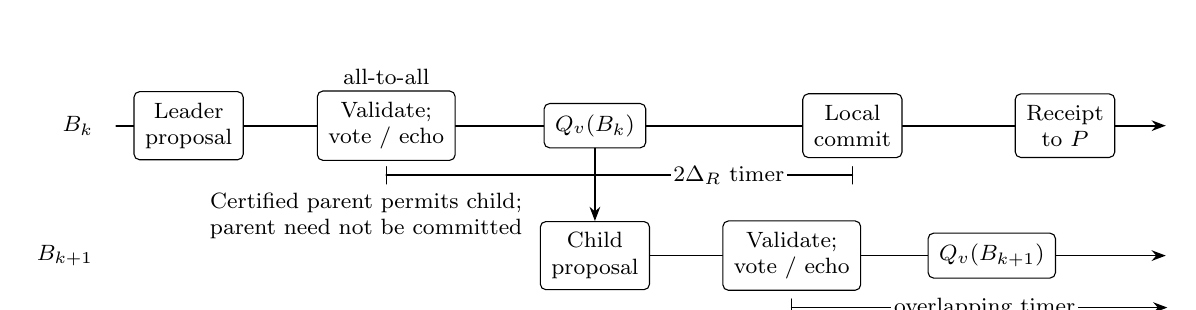
\begin{tikzpicture}[
  x=1cm,y=1cm,font=\footnotesize,line cap=round,line join=round,
  flow/.style={-{Stealth[length=1.8mm]},semithick},
  event/.style={draw,rounded corners=2pt,align=center,fill=white,inner sep=4pt},
  lab/.style={fill=white,inner sep=1pt,align=center}
]
  \node[anchor=east] at (.48,2.55) {$B_k$};
  \draw[flow] (.65,2.55) -- (13.98,2.55);
  \node[event] (prop) at (1.57,2.55) {Leader\\proposal};
  \node[event] (vote) at (4.08,2.55) {Validate;\\vote / echo};
  \node[event] (qc) at (6.73,2.55) {$Q_v(B_k)$};
  \node[event] (commit) at (10.00,2.55) {Local\\commit};
  \node[event] (receipt) at (12.70,2.55) {Receipt\\to $P$};
  \node[lab] at (4.08,3.17) {all-to-all};
  \draw[semithick] (4.08,1.92) -- (10.00,1.92);
  \draw (4.08,1.81) -- (4.08,2.03);
  \draw (10.00,1.81) -- (10.00,2.03);
  \node[lab] at (8.43,1.92) {$2\Delta_R$ timer};

  \node[anchor=east] at (.48,.90) {$B_{k+1}$};
  \draw[flow] (6.73,.90) -- (13.98,.90);
  \node[event] (child) at (6.73,.90) {Child\\proposal};
  \node[event] (cvote) at (9.23,.90) {Validate;\\vote / echo};
  \node[event] (cqc) at (11.77,.90) {$Q_v(B_{k+1})$};
  \draw[flow] (qc.south) -- (child.north);
  \node[lab,anchor=east] at (5.85,1.40) {Certified parent permits child;\\parent need not be committed};
  \draw[semithick] (9.23,.24) -- (13.65,.24);
  \draw (9.23,.13) -- (9.23,.35);
  \draw[flow] (13.65,.24) -- (14.00,.24);
  \node[lab] at (11.68,.24) {overlapping timer};
\end{tikzpicture}

\caption{Certification advances the proposal chain while commitment timers
overlap. A vote certificate and a confirmed-stream receipt have different meanings.}
\label{fig:pipeline}
\end{figure}

\Cref{fig:pipeline-communication} expands this pipeline into the message flow
among four regional sequencers. The drawing does not assign them equal stake.
Vote certificates require weight $>2W_i/3$; post-commit receipts require
matching endorsements of weight $>W_i/3$.

\begin{figure}[H]\centering
% Four-member steady-state message sequence.  Time runs from top to bottom;
% vertical distances show causal order rather than measured network delay.
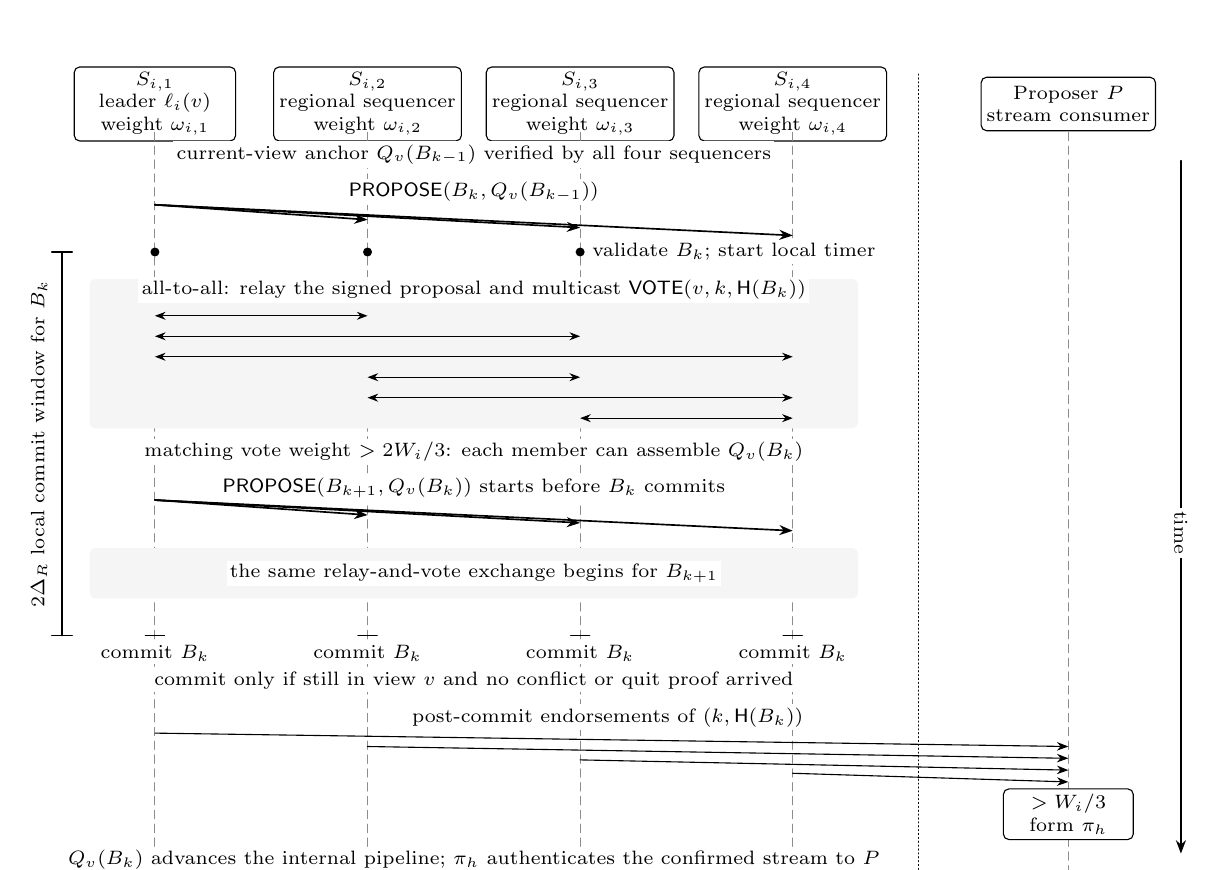
\begin{tikzpicture}[
  x=1cm,y=1cm,font=\scriptsize,line cap=round,line join=round,
  party/.style={draw,rounded corners=2pt,align=center,fill=white,
    minimum width=2.05cm,minimum height=.68cm,inner sep=2pt},
  lifeline/.style={densely dashed,thin,black!45},
  proposal/.style={-{Stealth[length=1.7mm]},semithick},
  exchange/.style={{Stealth[length=1.35mm]}-{Stealth[length=1.35mm]},thin},
  confirm/.style={-{Stealth[length=1.45mm]},thin},
  milestone/.style={circle,fill=black,inner sep=1.15pt},
  lab/.style={fill=white,inner sep=1.2pt,align=center}
]
  \def\xa{1.55}
  \def\xb{4.25}
  \def\xc{6.95}
  \def\xd{9.65}
  \def\xp{13.15}

  % Participants and lifelines.
  \node[party] at (\xa,10.30) {$S_{i,1}$\\leader $\ell_i(v)$\\weight $\omega_{i,1}$};
  \node[party] at (\xb,10.30) {$S_{i,2}$\\regional sequencer\\weight $\omega_{i,2}$};
  \node[party] at (\xc,10.30) {$S_{i,3}$\\regional sequencer\\weight $\omega_{i,3}$};
  \node[party] at (\xd,10.30) {$S_{i,4}$\\regional sequencer\\weight $\omega_{i,4}$};
  \node[party,minimum width=1.65cm] at (\xp,10.30)
    {Proposer $P$\\stream consumer};
  \foreach \x in {\xa,\xb,\xc,\xd,\xp}
    \draw[lifeline] (\x,9.94) -- (\x,.52);
  \draw[densely dotted] (11.25,10.68) -- (11.25,.45);
  \draw[proposal] (14.58,9.58) -- node[lab,right,rotate=-90] {time} (14.58,.78);

  % The current-view anchor is already common before the next proposal.
  \node[lab] at (5.60,9.66)
    {current-view anchor $Q_v(B_{k-1})$ verified by all four sequencers};

  % B_k proposal fan-out.
  \node[lab] at (5.60,9.18)
    {$\Tag{PROPOSE}(B_k,Q_v(B_{k-1}))$};
  \draw[proposal] (\xa,9.02) -- (\xb,8.83);
  \draw[proposal] (\xa,9.02) -- (\xc,8.73);
  \draw[proposal] (\xa,9.02) -- (\xd,8.63);
  \foreach \x in {\xa,\xb,\xc,\xd}
    \node[milestone] at (\x,8.42) {};
  \node[lab,anchor=east] at (10.75,8.42)
    {validate $B_k$; start local timer};

  % Explicit all-to-all exchange for B_k.  A bidirectional edge represents
  % the proposal relays and vote multicasts between that pair of members.
  \path[fill=black!4,rounded corners=2pt] (.72,6.18) rectangle (10.48,8.08);
  \node[lab] at (5.60,7.94)
    {all-to-all: relay the signed proposal and multicast $\Tag{VOTE}(v,k,\Hash(B_k))$};
  \draw[exchange] (\xa,7.61) -- (\xb,7.61);
  \draw[exchange] (\xa,7.35) -- (\xc,7.35);
  \draw[exchange] (\xa,7.09) -- (\xd,7.09);
  \draw[exchange] (\xb,6.83) -- (\xc,6.83);
  \draw[exchange] (\xb,6.57) -- (\xd,6.57);
  \draw[exchange] (\xc,6.31) -- (\xd,6.31);

  % Every member sees the multicast votes; certification immediately opens
  % the next pipeline position even though B_k's timers are still running.
  \foreach \x in {\xa,\xb,\xc,\xd}
    \node[milestone] at (\x,5.88) {};
  \node[lab] at (5.60,5.88)
    {matching vote weight $>2W_i/3$: each member can assemble $Q_v(B_k)$};

  \node[lab] at (5.60,5.43)
    {$\Tag{PROPOSE}(B_{k+1},Q_v(B_k))$ starts before $B_k$ commits};
  \draw[proposal] (\xa,5.27) -- (\xb,5.08);
  \draw[proposal] (\xa,5.27) -- (\xc,4.98);
  \draw[proposal] (\xa,5.27) -- (\xd,4.88);

  \path[fill=black!4,rounded corners=2pt] (.72,4.02) rectangle (10.48,4.66);
  \node[lab] at (5.60,4.34)
    {the same relay-and-vote exchange begins for $B_{k+1}$};

  % The B_k commit window overlaps communication for B_{k+1}.
  \draw[semithick] (.37,8.42) -- (.37,3.55);
  \draw[semithick] (.24,8.42) -- (.50,8.42);
  \draw[semithick] (.24,3.55) -- (.50,3.55);
  \node[lab,rotate=90] at (.08,5.98) {$2\Delta_R$ local commit window for $B_k$};
  \foreach \x in {\xa,\xb,\xc,\xd} {
    \draw[semithick] ($(\x,3.55)+(-.12,0)$) -- ($(\x,3.55)+(.12,0)$);
    \node[lab,anchor=north] at (\x,3.48) {commit $B_k$};
  }
  \node[lab] at (5.60,2.98)
    {commit only if still in view $v$ and no conflict or quit proof arrived};

  % Post-commit endorsements expose the committed prefix to P.  The leader
  % need not wait for this consumer-facing receipt before extending the chain.
  \node[lab] at (7.30,2.51)
    {post-commit endorsements of $(k,\Hash(B_k))$};
  \draw[confirm] (\xa,2.31) -- (\xp,2.14);
  \draw[confirm] (\xb,2.14) -- (\xp,1.99);
  \draw[confirm] (\xc,1.97) -- (\xp,1.84);
  \draw[confirm] (\xd,1.80) -- (\xp,1.69);
  \node[party,minimum width=1.65cm,minimum height=.52cm] at (\xp,1.28)
    {$>W_i/3$\\form $\pi_h$};
  \node[lab] at (5.60,.70)
    {$Q_v(B_k)$ advances the internal pipeline; $\pi_h$ authenticates the confirmed stream to $P$};
\end{tikzpicture}

\caption{Four-sequencer steady-state communication in one regional view.
The all-to-all exchange certifies $B_k$ and immediately enables its child while
the parent timers continue. Post-commit endorsements later expose a distinct
confirmed-stream receipt to $P$. Vertical positions show causal order, not
delay to scale.}
\label{fig:pipeline-communication}
\end{figure}

\subsection{Leader replacement and safe inheritance}
A view changes after lack of progress or authenticated leader equivocation,
not after an imposed batch quota. \Cref{alg:change} follows the four
view-change steps in Figure 2 of Sync HotStuff~\cite{synchotstuff}.
Write $\langle m\rangle_S$ for a message signed by member $S$, binding the
region and session as in \cref{sec:model}. Broadcast means send to
all regional members. Certificates travel with their blocks and any missing
ancestry needed for verification. At equal timestamps, process received
messages before testing deadlines.

\begin{protocol}{alg:change}{Regional view change from $v$ to $v+1$}
Let $L=\ell_i(v)$ and $L'=\ell_i(v+1)$. Each member $S$ records its entry
time $t_S(u)$ and entry-lock certificate $\mathit{lock}_S(u)$ for view $u$.
\begin{enumerate}[label=\textbf{V\arabic*.},itemsep=4pt]
\item \textbf{Blame and quit.} For each integer $p\geq1$, at time
$t_S(v)+(2p+4)\Delta_R$, if fewer than $p$ distinct fresh proposals have
triggered $S$'s votes in view $v$ (\textbf{missing blocks}), or propose pre-defined block upperbound(e.g., 100 batches) (\textbf{regular in-region rotation}), broadcast $\langle\Tag{BLAME},v\rangle_S$.
Anchor re-certification and duplicate messages do not count.
Quit view $v$ upon either of the following events:
\begin{itemize}
\item Receive BLAME signatures for $v$ from distinct members of total
weight $>W_i/3$: broadcast this blame certificate.
\item Detect leader equivocation: broadcast the two messages signed by $L$.
These are \Tag{PROPOSE}/\Tag{NEWVIEW} messages identifying conflicting blocks,
or two \Tag{NEWVIEW} messages selecting different anchors in view $v$.
\end{itemize}
Either witness is a \emph{quit proof}. On quitting, stop voting in $v$ and
cancel all its pending commit timers; retain every completed commitment.

\item \textbf{Status and entry.} Wait $\Delta_R$ \emph{from quitting},
continuing to collect old-view votes and certificates. Then choose a
highest-ranked valid certificate $Q=Q_{v'}(B_k)$ known to $S$, with $v'\leq v$;
set $\mathit{lock}_S(v+1)\gets Q$, send
$\langle\Tag{STATUS},v+1,Q\rangle_S$ to $L'$, and enter view $v+1$.
Record the entry time as $t_S(v+1)$ and keep this lock fixed throughout the view.

\item \textbf{New-view announcement (leader $L'$).} At time
$t_{L'}(v+1)+2\Delta_R$, choose a highest-ranked valid earlier-view
certificate $Q^*=Q_{v^*}(B_{k^*})$ known to $L'$, including its own status
and the received statuses, and broadcast
\[
 \langle\Tag{NEWVIEW},v+1,Q^*\rangle_{L'}.
\]
Announce only one anchor for this view.

\item \textbf{First vote (each member $S$).} In view $v+1$, on receiving
the above signed NEWVIEW directly or by relay, validate $B_{k^*}$ and $Q^*$.
If no leader equivocation is known, this is $S$'s first accepted NEWVIEW,
and
\[
 v^*<v+1,
 \qquad \rank(Q^*)\geq\rank\bigl(\mathit{lock}_S(v+1)\bigr),
\]
forward NEWVIEW to all members and broadcast
$\langle\Tag{VOTE},B_{k^*},v+1\rangle_S$.
This re-certifies the \emph{unchanged inherited block}; it starts no commit
timer. Once $L'$ obtains $Q_{v+1}(B_{k^*})$, it resumes
\cref{alg:steady} by proposing a fresh child of $B_{k^*}$.
\end{enumerate}
\end{protocol}

The two waits serve different purposes. The $\Delta_R$ wait after quitting
allows certificates protecting earlier commitments to be collected before
the next entry lock is fixed. Relaying a quit proof makes correct members'
entry times differ by at
most $\Delta_R$; the new leader's $2\Delta_R$ wait therefore covers that
entry skew and delivery of every correct member's STATUS. The selected
certificate can then meet every correct entry lock. The deadline index $p$
allows indefinite progress in one view; it is not a batch quota.

View entry requires the preceding quit proof. Buffer future-view messages
until entry and the required ancestry have been verified. Entry locks never
decrease in rank across views. Late old-view certificates are retained for
later recovery, but do not revise the current entry lock or an announced anchor.
For the initial view $0$, use the common checkpoint as the distinguished
certificate of rank $(-1,0)$ and as every member's entry lock, then run
steps V3--V4 with leader $\ell_i(0)$ and NEWVIEW for view $0$.
Initial participants are ready within $\Delta_R$ of one another.

\Cref{fig:change} expands the blame and recovery path into its communication
steps. The lanes show representative members of the same region; neither
four participants nor equal stake is assumed. In the figure, $Q_a$ and
$Q_b$ are the certificates selected as entry locks by members $S_{i,a}$
and $S_{i,b}$, respectively.

\begin{figure}[p]\centering
\resizebox{\linewidth}{!}{% Native TikZ fragment for main_v2.tex, Protocol V1--V4.
% All lanes belong to region V_i; arrows are representative transmissions.
% Bounding box: 15.8 cm by 20.3 cm before optional linewidth scaling.
% Explicit line breaks and fixed diagram fonts keep the layout independent
% of the surrounding document's base font size.
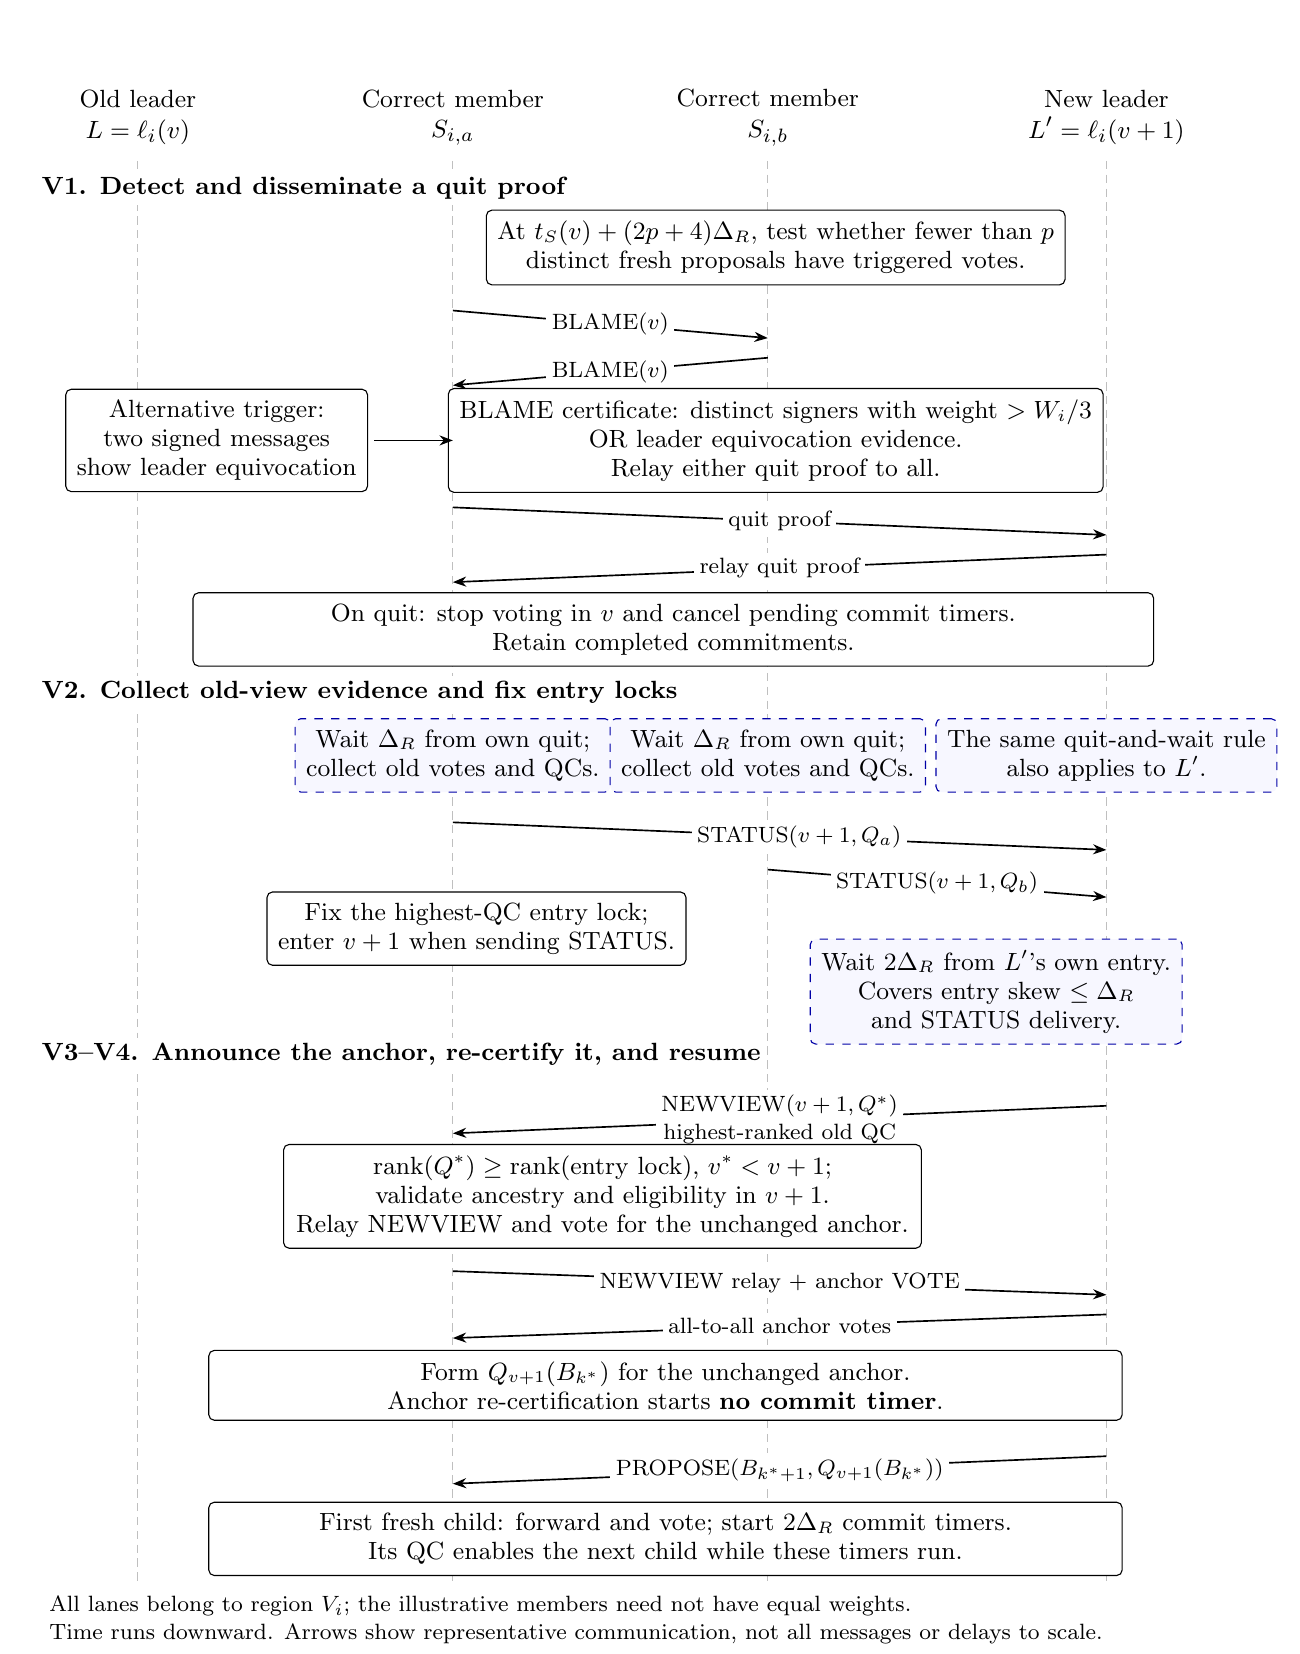
\begin{tikzpicture}[
  x=1cm,y=-1cm,font=\fontsize{9.5}{11}\selectfont,
  msg/.style={-{Stealth[length=1.7mm]},semithick},
  lane/.style={draw=black!25,densely dashed},
  label/.style={fill=white,inner sep=2pt,align=center,
    font=\fontsize{8.5}{10}\selectfont},
  phase/.style={anchor=west,font=\fontsize{9.5}{11}\selectfont\bfseries,
    fill=white,inner sep=2pt},
  state/.style={draw,rounded corners=2pt,fill=white,align=center,
    inner sep=4pt,font=\fontsize{9}{10.5}\selectfont},
  wait/.style={draw=blue!65!black,dashed,rounded corners=2pt,
    fill=blue!3,align=center,inner sep=4pt,
    font=\fontsize{9}{10.5}\selectfont}
]
  \path[use as bounding box] (-.4,-.65) rectangle (15.4,19.65);
  \node[align=center] at (1.0,0) {Old leader\\$L=\ell_i(v)$};
  \node[align=center] at (5.0,0) {Correct member\\$S_{i,a}$};
  \node[align=center] at (9.0,0) {Correct member\\$S_{i,b}$};
  \node[align=center] at (13.3,0) {New leader\\$L'=\ell_i(v+1)$};
  \foreach \x in {1,5,9,13.3} \draw[lane] (\x,.55)--(\x,18.65);

  \node[phase] at (-.3,.90) {V1. Detect and disseminate a quit proof};
  \node[state] at (9.1,1.65)
    {At $t_S(v)+(2p+4)\Delta_R$, test whether fewer than $p$\\
     distinct fresh proposals have triggered votes.};
  \draw[msg] (5,2.45)--node[label] {$\mathrm{BLAME}(v)$} (9,2.80);
  \draw[msg] (9,3.05)--node[label] {$\mathrm{BLAME}(v)$} (5,3.40);
  \node[state] at (2.0,4.10)
    {Alternative trigger:\\two signed messages\\show leader equivocation};
  \node[state,minimum width=7.8cm] at (9.1,4.10)
    {BLAME certificate: distinct signers with weight $>W_i/3$\\
     OR leader equivocation evidence.\\Relay either quit proof to all.};
  \draw[msg] (4.0,4.10)--(5.0,4.10);
  \draw[msg] (5,4.95)--node[label] {quit proof} (13.3,5.30);
  \draw[msg] (13.3,5.55)--node[label] {relay quit proof} (5,5.90);
  \node[state,minimum width=12.2cm] at (7.8,6.50)
    {On quit: stop voting in $v$ and cancel pending commit timers.\\
     Retain completed commitments.};

  \node[phase] at (-.3,7.30) {V2. Collect old-view evidence and fix entry locks};
  \node[wait] at (5,8.10)
    {Wait $\Delta_R$ from own quit;\\collect old votes and QCs.};
  \node[wait] at (9,8.10)
    {Wait $\Delta_R$ from own quit;\\collect old votes and QCs.};
  \node[wait] at (13.3,8.10)
    {The same quit-and-wait rule\\also applies to $L'$.};
  \draw[msg] (5,8.95)--node[label,pos=.53] {$\mathrm{STATUS}(v+1,Q_a)$} (13.3,9.30);
  \draw[msg] (9,9.55)--node[label] {$\mathrm{STATUS}(v+1,Q_b)$} (13.3,9.90);
  \node[state] at (5.3,10.30)
    {Fix the highest-QC entry lock;\\enter $v+1$ when sending STATUS.};
  \node[wait] at (11.9,11.10)
    {Wait $2\Delta_R$ from $L'$'s own entry.\\
     Covers entry skew $\leq\Delta_R$\\and STATUS delivery.};

  \node[phase] at (-.3,11.90) {V3--V4. Announce the anchor, re-certify it, and resume};
  \draw[msg] (13.3,12.55)--node[label,pos=.50]
    {$\mathrm{NEWVIEW}(v+1,Q^*)$\\highest-ranked old QC} (5,12.90);
  \node[state,minimum width=8.1cm] at (6.9,13.70)
    {$\operatorname{rank}(Q^*)\geq\operatorname{rank}(\mathrm{entry\ lock})$,
     $v^*<v+1$;\\validate ancestry and eligibility in $v+1$.\\
     Relay NEWVIEW and vote for the unchanged anchor.};
  \draw[msg] (5,14.65)--node[label] {NEWVIEW relay + anchor VOTE} (13.3,14.95);
  \draw[msg] (13.3,15.20)--node[label] {all-to-all anchor votes} (5,15.50);
  \node[state,minimum width=11.6cm] at (7.7,16.10)
    {Form $Q_{v+1}(B_{k^*})$ for the unchanged anchor.\\
     Anchor re-certification starts \textbf{no commit timer}.};
  \draw[msg] (13.3,17.00)--node[label,pos=.50]
    {$\mathrm{PROPOSE}(B_{k^*+1},Q_{v+1}(B_{k^*}))$} (5,17.35);
  \node[state,minimum width=11.6cm] at (7.7,18.05)
    {First fresh child: forward and vote; start $2\Delta_R$ commit timers.\\
     Its QC enables the next child while these timers run.};
  \node[align=left,font=\fontsize{8.5}{10}\selectfont,anchor=west] at (-.25,19.08)
    {All lanes belong to region $V_i$; the illustrative members need not have equal weights.\\
     Time runs downward. Arrows show representative communication, not all messages or delays to scale.};
\end{tikzpicture}
}
\caption{Regional blame and view-change communication. A blame quorum or
leader-equivocation proof causes view exit. Each member waits $\Delta_R$
from its own exit before sending STATUS; the new leader waits $2\Delta_R$
from its own entry before announcing NEWVIEW. Re-certifying the unchanged
anchor starts no commit timer; the first fresh child resumes the pipeline.
Time runs downward, and arrows show representative transmissions.}
\label{fig:change}
\end{figure}

The list $\mathcal L_i$ specifies who replaces a failed producer inside
this region. Cross-region quota expiry uses a finalized application anchor,
not a fabricated local BLAME event; it is defined in \cref{sec:rotation}.

\subsection{Application quota and terminal drain}\label{sec:drain}
The physical SMR log uses two block types. An \Tag{APP} block contributes
one application batch to the stream; a \Tag{DRAIN} block contributes no
application batch, mini-block or transaction. Both bind their type, parent,
physical position and session, and follow the same proposal, vote, timer
and view-change rules. A DRAIN block has no ORDER headers to sign.

\begin{protocol}{alg:drain}{Quota adapter and terminal completion}
\begin{enumerate}[label=\textbf{Q\arabic*.}]
\item \textbf{Validate the proposed ancestry.} Count application blocks
from the session anchor, including uncommitted proposed ancestors. Reject
an APP block if this count would exceed $K$. Counting only committed
blocks would permit pipelined overshoot.
\item \textbf{Finish the application segment.} While the count is below
$K$, use APP blocks. Every APP binds the L1 reference of
\cref{sec:snapshot}; the $K$th one is terminal and its reference determines
the regular handoff's initial control height. Once a proposed chain reaches $K$,
all fresh descendants on that chain are DRAIN blocks.
DRAIN does not advance the application timestamp or postpone a scheduled
retirement; forced closure remains governed by \cref{ass:recovery}.
\item \textbf{Maintain native progress.} Both APP and DRAIN proposals
count in the deadline index $p$ of \cref{alg:change}. After NEWVIEW,
if the inherited chain already has $K$ application blocks, propose a
fresh DRAIN child; its normal commit timer also commits its ancestors.
Otherwise complete the remaining application positions.
\item \textbf{Export and retire.} Once a terminal application receipt
is verified, retain and relay its complete application prefix, ancestry
and receipt; stop new physical proposals, votes and progress timers in this
completed session. Keep the fetch service and signing history. The wrapper
may wait for a successor without running more DRAIN blocks. No later physical output
from this closed session is accepted as a new application batch.
\end{enumerate}
\end{protocol}
This adapter leaves the native commit test unchanged. Application projection
preserves physical-log safety. Under regional progress, a terminal batch
receives its own commitment or is committed by a DRAIN descendant; it
cannot be stranded solely because NEWVIEW re-certification starts no timer.
There is no fixed bound on control descendants through arbitrarily many
failed views. In a healthy view, the terminal batch's own timer normally
finishes without an extra finalization round. An unavailable successor
may keep the wrapper waiting at this fixed terminal prefix; it does not
extend the old application quota.

\smallskip
\Needspace{9\baselineskip}
\noindent\textbf{Example: completing a three-batch term.}
Let $K=3$ and let a session start at $A_{100}$, whose last mini-block
height is $300$. Its first three physical blocks are APP blocks:
$B_1$ carries $X_{101}$ with mini-blocks $301$--$303$,
$B_2$ carries $X_{102}$ with mini-blocks $304$--$305$, and
$B_3$ carries terminal batch $X_{103}$ with mini-block $306$ and the
bound L1 reference $\rho_{103}$. All mini-blocks of each $X_b$ carry its
common timestamp $L_b$, with $L_{101}\leq L_{102}\leq L_{103}$.
The proposed ancestry already contains three APP blocks, even if some
remain uncommitted. Thus Q1--Q2 reject a fourth APP on this chain;
any fresh child of $B_3$ must be DRAIN.

Suppose $Q_v(B_3)$ has formed, but a quit proof cancels the pending
timers before $B_3$ commits, and view $v+1$ inherits $B_3$.
NEWVIEW re-certifies this unchanged block as $Q_{v+1}(B_3)$ without
starting a commit timer. By Q3, the new leader proposes a fresh DRAIN
child $B_4$. Its normal $2\Delta_R$ timer starts on validation and voting;
if it expires in view $v+1$ without equivocation, the member commits
$B_4$ and its uncommitted ancestors, including $B_3$.
Post-commit confirmations then supply $F_{103}$. On verifying that
receipt, Q4 exports
$A_{103}=(103,306,\Hash(X_{103}),q_{306})$ and retires the session's
physical pipeline while preserving retrieval.
The DRAIN child occupies $k=4$ but adds no application position:
the completed term ends at $(b,h,d)=(103,306,3)$.
\Cref{fig:terminal-drain} shows this recovery path. If $B_3$ instead
commits on its own timer in a healthy view, export uses that commitment
without waiting for a DRAIN descendant to commit.

\begin{figure}[H]\centering
% One session, K=3. The physical chain and application projection are separate.
% The recovery path assumes NEWVIEW selects B_3 before B_3 has committed.
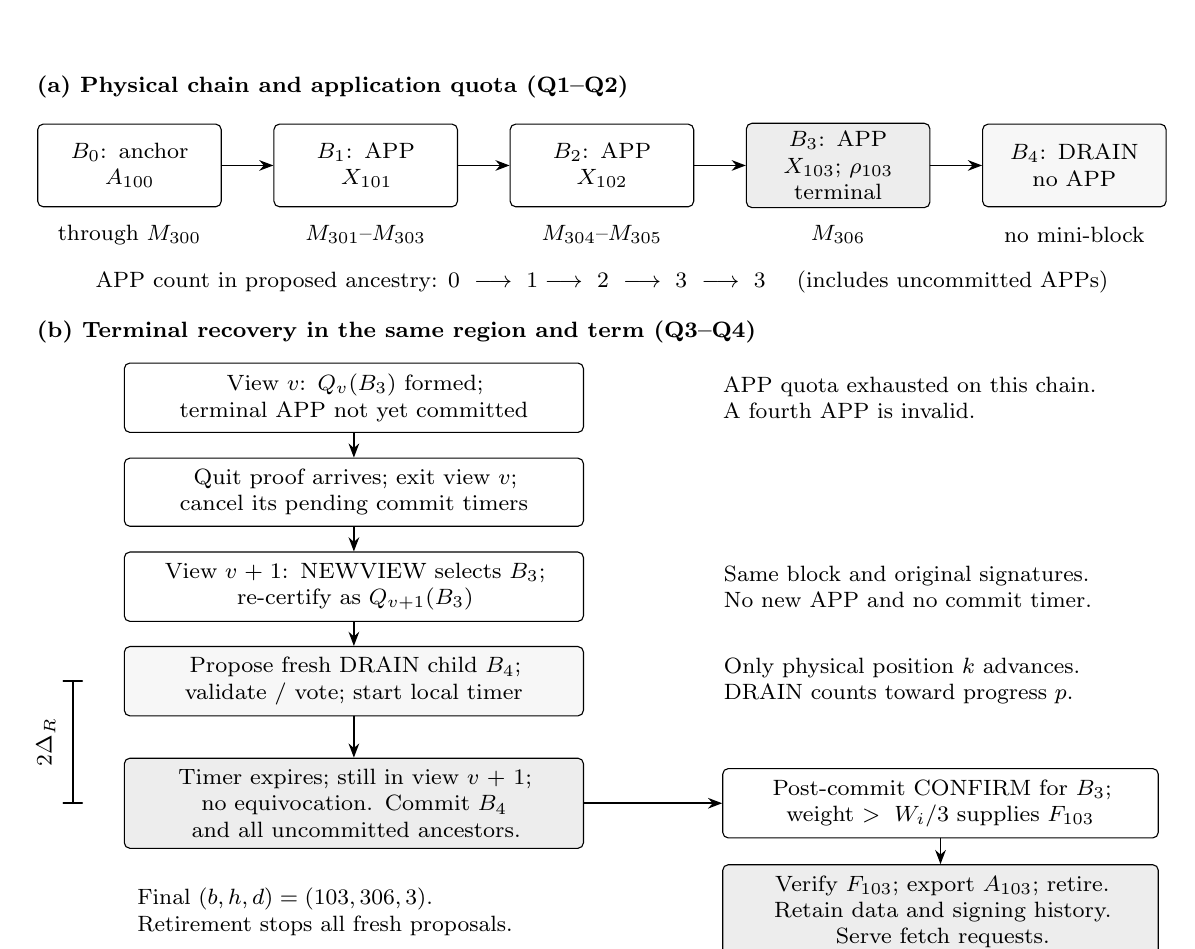
\begin{tikzpicture}[
  x=1cm,y=1cm,font=\footnotesize,line cap=round,line join=round,
  flow/.style={-{Stealth[length=1.8mm]},semithick},
  block/.style={draw,rounded corners=2pt,fill=white,align=center,
    text width=2.12cm,minimum height=1.05cm,inner sep=3pt},
  event/.style={draw,rounded corners=2pt,fill=white,align=center,
    text width=5.55cm,minimum height=.75cm,inner sep=4pt},
  note/.style={align=left,text width=5.5cm,inner sep=3pt},
  lab/.style={fill=white,inner sep=2pt,align=center}
]
  \node[anchor=west,font=\footnotesize\bfseries] at (0,1.00)
    {(a) Physical chain and application quota (Q1--Q2)};
  \node[block] (root) at (1.30,0)
    {$B_0$: anchor\\$A_{100}$};
  \node[block] (appone) at (4.30,0)
    {$B_1$: APP\\$X_{101}$};
  \node[block] (apptwo) at (7.30,0)
    {$B_2$: APP\\$X_{102}$};
  \node[block,fill=black!7] (terminal) at (10.30,0)
    {$B_3$: APP\\$X_{103}$; $\rho_{103}$\\terminal};
  \node[block,fill=black!3] (drain) at (13.30,0)
    {$B_4$: DRAIN\\no APP};
  \draw[flow] (root) -- (appone);
  \draw[flow] (appone) -- (apptwo);
  \draw[flow] (apptwo) -- (terminal);
  \draw[flow] (terminal) -- (drain);
  \node[lab] at (1.30,-.88) {through $M_{300}$};
  \node[lab] at (4.30,-.88) {$M_{301}$--$M_{303}$};
  \node[lab] at (7.30,-.88) {$M_{304}$--$M_{305}$};
  \node[lab] at (10.30,-.88) {$M_{306}$};
  \node[lab] at (13.30,-.88) {no mini-block};
  \node[lab] at (7.30,-1.48)
    {APP count in proposed ancestry: $0\ \longrightarrow\ 1
     \longrightarrow\ 2\ \longrightarrow\ 3\ \longrightarrow\ 3$
     \quad (includes uncommitted APPs)};

  \node[anchor=west,font=\footnotesize\bfseries] at (0,-2.12)
    {(b) Terminal recovery in the same region and term (Q3--Q4)};
  \node[event] (oldqc) at (4.15,-2.95)
    {View $v$: $Q_v(B_3)$ formed;\\terminal APP not yet committed};
  \node[note] at (11.60,-2.95)
    {APP quota exhausted on this chain.\\A fourth APP is invalid.};

  \node[event] (quit) at (4.15,-4.15)
    {Quit proof arrives; exit view $v$;\\cancel its pending commit timers};
  \draw[flow] (oldqc) -- (quit);

  \node[event] (newview) at (4.15,-5.35)
    {View $v+1$: NEWVIEW selects $B_3$;\\re-certify as $Q_{v+1}(B_3)$};
  \draw[flow] (quit) -- (newview);
  \node[note] at (11.60,-5.35)
    {Same block and original signatures.\\No new APP and no commit timer.};

  \node[event,fill=black!3] (fresh) at (4.15,-6.55)
    {Propose fresh DRAIN child $B_4$;\\validate / vote; start local timer};
  \draw[flow] (newview) -- (fresh);
  \node[note] at (11.60,-6.55)
    {Only physical position $k$ advances.\\DRAIN counts toward progress $p$.};

  \node[event,fill=black!7] (commit) at (4.15,-8.10)
    {Timer expires; still in view $v+1$;\\no equivocation. Commit $B_4$\\and all uncommitted ancestors.};
  \draw[flow] (fresh) -- (commit);
  \draw[semithick] (.58,-6.55) -- (.58,-8.10);
  \draw[semithick] (.46,-6.55) -- (.70,-6.55);
  \draw[semithick] (.46,-8.10) -- (.70,-8.10);
  \node[lab,rotate=90] at (.24,-7.325) {$2\Delta_R$};

  \node[event,text width=5.25cm] (receipt) at (11.60,-8.10)
    {Post-commit CONFIRM for $B_3$;\\weight $>W_i/3$ supplies $F_{103}$};
  \draw[flow] (commit) -- (receipt);

  \node[event,text width=5.25cm,fill=black!7] (retire) at (11.60,-9.48)
    {Verify $F_{103}$; export $A_{103}$; retire.\\Retain data and signing history.\\Serve fetch requests.};
  \draw[flow] (receipt) -- (retire);
  \node[note] at (4.15,-9.48)
    {Final $(b,h,d)=(103,306,3)$.\\Retirement stops all fresh proposals.};
\end{tikzpicture}

\caption{Quota enforcement and terminal recovery for $K=3$
(Protocol~\ref{alg:drain}, Q1--Q4). The upper chain shows physical blocks
and their application projection; the lower pipeline follows a view change
before the terminal APP commits. Re-certification starts no timer, whereas
a fresh DRAIN child can commit the terminal ancestor. Arrows show causal
order; the timer is local and the drawing is not to scale.}
\label{fig:terminal-drain}
\end{figure}

\subsection{Confirmation receipts and slashing}\label{sec:receipt}
After committing $B_k$, an honest member signs a CONFIRM statement binding
the session, block digest and position, and sends it to peers and subscribed
consumers. Matching CONFIRM endorsements from distinct members of weight
$>W_i/3$, with the block and any missing ancestry, form the receipt $\pi_h$
for its committed prefix. CONFIRM signatures are domain-separated from VOTE
and follow the local commit rule. A raw vote QC is not a receipt.

Let $D=(\mathit{chainId},\mathit{contract},\mathit{cfg},i,s)$ be the signing
domain: the chain identifier, adjudicating contract, fixed configuration
identifier, region and session identifier. Signed statements bind $D$ through their authorization
context. Headers use a canonical encoding; a mini-block's identity remains
$q_h=\Hash(\Tag{MINIBLOCK},H_h)$, independent of signature encoding.

\begin{definition}[Leader double-head evidence]\label{def:double-head}
Write $\operatorname{ctx}(H)=(D,v,h)$ for an ORDER header's authorization
context, original producing view and mini-block height. Let
$E=(H,H',\sigma,\sigma')$, where $\sigma$ and $\sigma'$ are signatures by
the same producer key $S$. Then $E$ is valid double-head evidence if
\[
 \begin{gathered}
 \operatorname{ctx}(H)=\operatorname{ctx}(H')=(D,v,h),
 \qquad S=\ell_i(v)\text{ in the configuration identified by }D,\\
 \operatorname{Verify}_{S}(\Tag{ORDER},H,\sigma)
 =\operatorname{Verify}_{S}(\Tag{ORDER},H',\sigma')=1,\\
 \Hash(\Tag{MINIBLOCK},H)\ne\Hash(\Tag{MINIBLOCK},H').
 \end{gathered}
\]
\end{definition}
The two authenticated headers suffice: the leader has signed different
heads for the same production opportunity, whether or not either was voted
on or committed. A different parent or transaction commitment changes the
head. No quorum certificate or proof of elapsed time is required.
The comparison uses the original producing view in the headers, not the view
of a later certificate that re-certifies their batch.

\begin{protocol}{alg:slash}{Submit and adjudicate leader double-head evidence}
\textbf{Input:} evidence $E$ and the configuration referenced by $D$.
\begin{enumerate}[label=\textbf{E\arabic*.}]
\item \textbf{Submit.} Any observer may submit the two original signed
headers to the L1 adjudicator.
\item \textbf{Verify.} Require $D$ to name this chain and adjudicating
contract. Resolve its session and historical configuration from the
contract's authorized records; check canonical encoding, producer
authorization and every condition of \cref{def:double-head}. Reject evidence
failing any check.
\item \textbf{Deduplicate.} Compute the offense identifier
\[
 o=\Hash(\Tag{DOUBLEORDER},D,S,v,h).
\]
Skip an already adjudicated $o$. This slot-level identifier prevents repeated
penalties from reordered evidence, alternative signatures or additional
conflicting heads at the same slot.
\item \textbf{Apply.} Atomically record $o$ and impose the configured L1
equivocation penalty on $S$. Retain the evidence; membership and weights
remain fixed until an authorized configuration transition.
\end{enumerate}
\end{protocol}

The remaining signed comparison domains protect the corresponding rules:
\begin{itemize}
\item \emph{Votes:} one member signs different block digests at the same
$D$, view and physical block position $k$.
\item \emph{Leader proposals:} one leader signs incompatible
PROPOSE/NEWVIEW blocks in the same $D$ and view, or announces two different
NEWVIEW anchors for that view. Two different anchors violate the single-anchor
rule even when one extends the other.
\item \emph{Confirmations:} one member endorses incompatible committed
prefixes in the same $D$, even if the endorsements originate in different
views. The evidence includes the signed endpoints and authenticated ancestry
needed to exhibit a conflicting position.
\end{itemize}
Evidence concerns the original signer; forwarding it or re-encoding a
signature does not create equivocation. Lawful cross-view re-proposals and
unchanged-anchor re-certification do not satisfy the same-view ORDER or VOTE
rules; incompatible confirmed prefixes remain evidence across views.
Silence and BLAME alone do not prove equivocation. L1 staking rules set
penalties, evidence retention and withdrawal conditions.
Status-entry signatures have their own committee domain and predecessor
version, defined next. They do not add a cross-region consensus vote to
the regional data path.


\section{Regional Status Committee}\label{sec:committee}
\subsection{Status entries with future activation heights}
For version $j\geq1$, let $a_j$ be a future L1 block height and let
$\chi_j:\mathcal R\to\{\Tag{live},\Tag{off}\}$ be a region-status map.
The committee authenticates the scheduled update
\[
 E_j=(a_j,\chi_j).
\]
The version $j$ counts entries, independently of the member index in
$S_{i,j}$. A live region is eligible for selection; this label does not
promise continued responsiveness. The committee schedules eligibility
changes, not application checkpoints or successor headers.

\Needspace{8\baselineskip}
For example, with regions $\mathcal R=\{A,B,C\}$, the entry
\[
 E_7=\bigl(1050,\{A\mapsto\Tag{live},\ B\mapsto\Tag{off},
 \ C\mapsto\Tag{live}\}\bigr)
\]
means that this map applies from L1 control height $1050$ until the next
scheduled update. Earlier control heights use the preceding map, even if
$E_7$ is already announced on L1. The number $1050$ is not an application
batch height and authenticates no batch contents. Such contents require
regional receipts and ancestry.

L1 installs the cyclic region list $\mathcal L_R$ and an initial entry
$E_0=(a_0,\chi_0)$ effective at the configured initial L1 origin. The first
live region in the list starts term $0$ at $A_0$ with application height $1$;
if none is live, initialization waits.
For $j\geq1$, the authenticated envelope is
\[
 \widehat E_j=(D_C,j,p_j,E_j,\Sigma_j^C),\qquad
 p_j=\Hash(\Tag{ENTRY},D_C,j-1,E_{j-1}).
\]
The signing domain $D_C$ names the chain, registry contract and committee
snapshot. All displayed fields are signed; signature encodings do not
change entry identity. Correct members persist their signing state and
endorse at most one successor for each predecessor and version. With
faulty committee stake below $W_C/3$ and certificate weight $>2W_C/3$,
conflicting certified successors require an honest double endorsement.
These weights are independent of the regional certificate thresholds.

\begin{assumption}[Ordered status service]\label[assumption]{ass:committee}
The committee produces a consistent authenticated entry history and
certifies admissible updates under its observation, coordination and
L1-submission conditions. L1 supplies a common finalized history. If an
entry is installed in L1 block $u_j$, the registry checks its domain,
certificate, consecutive version and predecessor, together with
\[
 a_j>a_{j-1},\qquad a_j\geq u_j+w_{\min},\qquad
 \chi_j\ne\chi_{j-1},
\]
where $w_{\min}>0$ is the configured minimum announcement distance in L1
blocks. Installed schedules are immutable; another update receives a new
version and a later activation height.
\end{assumption}
An entry may be installed well before it becomes effective. Only the latter
event changes eligibility. Committee coordination remains a separate
low-frequency task; threshold signatures alone do not specify its algorithm.

\subsection{Announcement, preparation and effective updates}
The committee observes sustained lack of progress, reachability and
recovery reports. These observations support status changes, not automatic
equivocation penalties. A recovering region obtains the current
configuration and finalized data before being scheduled live again.

\begin{protocol}{alg:status}{Schedule and apply a regional status update}
\begin{enumerate}[label=\textbf{C\arabic*.}]
\item \textbf{Schedule.} Construct a changed map and select a future
activation height $a_j$ satisfying the announcement policy. Keep regional
membership and the installed region order unchanged. The entry specifies
no application retirement cutoff.
\item \textbf{Certify and install.} Authenticate the next envelope. Any
relayer may submit it; the registry performs the checks above. Distribute
its L1 inclusion and finality proofs. Installation alone changes neither
the current session nor its quota.
\item \textbf{Prepare.} During the notice window, synchronize eligible
successors, retain application data and receipts, and prepare safe closure
of any authority that may be retired. Already authorized production may
continue subject to quota and the admission rules in \cref{sec:snapshot}.
\item \textbf{Apply when due.} Process the entry only at control height
$a_j$, after L1 finality through that height. Classify it against the
certified authority at this boundary, which may differ from the authority
at announcement. If that region remains live, update eligibility only.
If it becomes off, latch a forced-handoff obligation; safe closure and
recovery must complete before a successor starts.
\end{enumerate}
\end{protocol}
An inactive region's recovery leaves a healthy current term unchanged.
It may enable an already waiting handoff once its scheduled height is
reached. A later live update does not revive a retired session or erase an
outstanding forced-handoff obligation.

The height distance $w_{\min}$ is not by itself a bound on usable preparation
time. For timing guarantees, assume that every relevant serving participant
can authenticate the announcement at least $T_{\rm prep}$ before the
activation boundary can be acted upon. This lead time must account for L1
finality and control-proof dissemination; advancing several finalized L1
heights at once does not create elapsed preparation time. The deployment
must justify this notice condition from its L1 and network assumptions.
If notice or recovery is insufficient, the wrapper waits at the required
boundary; it does not roll back a confirmed prefix or fabricate a cut.

\subsection{L1 timestamps, effective maps and handoff boundaries}\label{sec:snapshot}
L1 supplies one ordered schedule. For a finalized L1 control height $L$,
the effective version and map are
\[
 j(L)=\max\{j:a_j\leq L\},\qquad \chi_{\rm eff}(L)=\chi_{j(L)}.
\]
A batch's signed timestamp $L_b$ determines which entries are due; neither
its producer nor a later receiver chooses a different status version at
that height. Each batch carries, or references cached evidence for,
\[
 \rho_b=(L_b,r_b,R_b,J_b),
\]
where $r_b$ is the canonical L1 block hash, $R_b$ its authenticated registry
root, and $J_b$ the last entry installed there. The proof authenticates the
complete entry prefix through $J_b$. Installed entries with $a_j>L_b$
remain pending: $J_b$ need not equal $j(L_b)$.

For example, suppose $E_6$ makes $B$ live and the announced $E_7$ above makes
$B$ off at $1050$. A batch timestamped $1049$ still uses $E_6$; one
at $1050$ uses $E_7$. With region order $(A,B,C)$, a regular handoff from
$A$ at the former height selects $B$, while one at the latter selects $C$.
If $B$ takes over at $1049$, the update at $1050$ is evaluated against $B$
and may require another handoff; it does not rewrite the earlier choice.
Historical verification always uses the signed height, even after further
L1 updates. Multiple batches may share one height, and all mini-blocks of
a batch share its reference.

\noindent\textbf{Fresh admission and control progress.}
A leader attaches its latest verified finalized L1 reference when forming
a fresh APP. Members check the finality and registry proofs, equality of
the batch's mini-block references, nondecreasing timestamps, and the
session's authority after replaying all entries due at that timestamp.
A fresh APP that would cross an update retiring its session is rejected.
This historical validity test is identical at all replicas; a receiver's
newer local L1 head does not change it. Inherited blocks, in-flight
commitments and historical receipts retain their original timestamps.

The wrapper watches finalized L1 independently of APP production. Its
control cursor must eventually advance through newly finalized activation
heights, even if the application stream has stopped. A due retirement
initiates closure of the affected authority independently of the timestamps
its leader proposes. Closure must reconcile commitments and pending work
under \cref{ass:recovery}; a local L1 observation alone is not a new native
quit proof or permission to silently stop voting while others commit.
Once closure is certified, fresh work from the retired session is rejected
even if it carries an old timestamp. Thus timely retirement relies on
control progress and fencing, not on header monotonicity alone.
While a session remains in service and its required proofs are available,
the ordinary regional pipeline is unchanged.

A regular handoff initially uses the terminal batch's $L_b$ and
$\chi_{\rm eff}(L_b)$. A waiting boundary can advance its authenticated
control cursor as later entries become effective, without changing the
terminal batch or its timestamp. It is \emph{sealed} once its boundary
evidence fixes a successor and selection height. A later update is applied
to that successor; it never reselects the old boundary. When a scheduled
update and a quota boundary have the same control height, process the
update first. Control witnesses record this order, including advances
that occur without an APP.

An activation height $a_j$ is not an application cutoff. Forced recovery
separately determines a batch height $\beta_*$ and its finalized anchor
$A_{\beta_*}$. The old session may have produced additional final batches
during the notice window. A \emph{closed cut} preserves them and closes all
competing old authority before the successor starts.

\begin{assumption}[Admissible control and recovery cuts]\label[assumption]{ass:recovery}
Control-cursor advances and sealed regional handoffs have an authenticated
common order. A due retirement at $a_{j_*}$ is evaluated against the unique
authority at that boundary. Its recovery witness binds the triggering entry,
retiring session, control history and one application cut $\beta_*$,
satisfying all of the following:
\begin{enumerate}[label=(\roman*)]
\item every completed honest application commitment, every delivered
prefix, and every prefix for which a final receipt can already be assembled
under affected authority is a prefix of $A_{\beta_*}$;
\item affected old authority, including a concurrently issued successor
authority, is fenced: it cannot later create an accepted application
continuation outside the new authorized path, including through fresh
proposals carrying an old L1 timestamp;
\item the anchor's bytes, receipts and missing ancestry are recoverable;
\item the witness cannot authorize a competing successor to an already
sealed handoff. The effective control prefix and currently authorized
session are unambiguous, and each retired session has one accepted cut.
\end{enumerate}
Closure preserves native regional commitment and view-change guarantees:
it reconciles pending work before fencing, rather than changing proposal
validity separately at different replicas. This control/engine integration
is part of the recovery premise.
A sealed normal handoff fixes its selection height permanently. Subsequent
updates are evaluated against its certified successor. The new session's
opening height is at least the cut's last application timestamp and the
height of the control transition that authorizes the session.
\end{assumption}
These recovery conditions require evidence beyond a schedule or elapsed
window. For example, if the stream advances from batch 100 to finalized
batch 105 during preparation, a cutoff at 100 is invalid even if 105 has
not reached L1 publication. Recovery must preserve the higher prefix and
close the old authority. If a complete safe cut or its data is unavailable,
new-region production waits. L1-height timestamps specify control context;
they do not prove when a signature was physically created or that no hidden
higher final receipt exists.

\section{Cross-Region Rotation}\label{sec:rotation}
\subsection{Selection and derived authority}
For the installed cyclic list, define
\[
 \Proc{NextLive}(i,\chi)=\text{first other region after $i$ in
 $\mathcal L_R$ whose status is live}.
\]
Search at most one traversal. If no such region exists, the result is
$\bot$ (no eligible successor) and the wrapper waits. Same-region renewal is not counted
as a cross-region rotation. The committee changes eligibility through its
map; it does not choose an arbitrary successor or alter the producer list.

\Needspace{13\baselineskip}
The verifier maintains the accepted checkpoint and cached history introduced
in \cref{sec:xstream}. Its derived control state is
\[
 \mathcal Z=(\alpha,b,d,L_{\rm c},j_{\rm a},\chi,\mathit{phase},\mathit{pending}),
\]
where $\alpha$ is the immutable current session context, $b$ is the last
accepted global application height, $d$ is the number of application batches
accepted in this term, $L_{\rm c}$ is the authenticated control cursor,
and $j_{\rm a}=j(L_{\rm c})$ is the last effective status version processed.
The map $\chi=\chi_{\rm eff}(L_{\rm c})$ records effective eligibility;
future installed entries are cached separately. The phase is active while the
session serves and waiting while a handoff is pending. The field
$\mathit{pending}$ stores an outstanding forced-handoff obligation, if any.
Control advances and passive updates may advance $L_{\rm c}$, $j_{\rm a}$ and
$\chi$ without changing $\alpha$ or $d$. This is derived verifier state,
not additional committee-maintained state.

At one \emph{unsealed authenticated boundary}, process newly due entries
one at a time, in activation order. The first making the then-active
region off latches
$\mathit{pending}=(j_*,a_{j_*},\alpha_*)$, retaining the triggering entry,
activation height and retiring session. Its application cut is initially
unresolved; once verified, the recovery witness fixes $\beta_*$.
Later effective entries can update successor eligibility but cannot erase
this obligation or replace an accepted cut. If a forced
obligation is pending, use the forced path; otherwise, if $d=K$, use the
regular path; otherwise continue the current region.
The priority applies only under \cref{ass:recovery}. It is not a rule that a
late failure report may overwrite a previously sealed regular transition.
Each installed transition increments $\tau$, creates one new session and
resets $d$; merely applying an entry does none of these things.

\subsection{Regular term expiry}\label{sec:regular}
A regular term expires after its fixed quota, not after a receiver's local
wall-clock timeout. This is the scheduled or term-expiry cross-region path.
A data-fetch timeout or a silent-producer timeout can request observation
or local recovery, but cannot by itself grant another region authority.

\begin{protocol}{alg:regular}{Regular cross-region handoff}
\textbf{Input:} the current session has admitted $K$ application batches.
\begin{enumerate}[label=\textbf{R\arabic*.}]
\item \textbf{Finish.} Complete \Proc{Drain}; obtain terminal batch $X_b$,
its post-commit receipt $F_b$, ancestry and its bound L1 reference $\rho_b$.
The previous input prefix is preserved byte for byte.
\item \textbf{Derive.} Verify $K$ application positions and the complete
registry prefix at $L_b$. Replay entries effective by this height and any
already ordered boundary control advances. Apply a due update before quota
expiry at the same height. If force is due, use \cref{alg:force};
otherwise set $i'=\Proc{NextLive}(i,\chi_{\rm eff}(L_{\rm c}))$.
\item \textbf{Wait or seal.} If $i'=\bot$, retain this fixed terminal
anchor and its unchanged timestamp. Process later effective entries in
authenticated order; the first admissible control
prefix that enables a valid successor completes the pending handoff.
Otherwise the valid terminal and control witnesses seal that successor
and its selection height $L_{\rm c}$.
Receivers do not reselect it using later maps.
\item \textbf{Transfer and open.} A retained holder sends $A_b,F_b$,
contents, ancestry and control evidence to region $i'$. It verifies the
regional interface and new authority, then atomically installs the new
$\alpha$ with $L_0=L_{\rm c}$ and $j_0=j(L_{\rm c})$, sets $d=0$ and phase active, clears pending boundary metadata,
and opens the new session at $A_b$.
Prewarming may transfer data earlier but cannot start ordering on an
unfinalized anchor.
\item \textbf{Continue.} The first new application batch is $b+1$;
its first mini-block has predecessor $q_h$ and height $h+1$ from $A_b$,
and the batch timestamp is at least $L_0$. Any further due update is
processed against this new session before admitting that batch.
Run the new regional SMR and deliver its confirmed outputs through
\Proc{VerifyCross}. No separate cross-region vote is added per batch.
\end{enumerate}
\end{protocol}
A new committee entry is not required merely because $K$ batches elapsed.
The old region finalizes its terminal batch without waiting for the new
region to finalize a child. This removes circular handoff dependencies.

\begin{figure}[htbp]\centering
% Time flows down. The old region finalizes before the new one proposes.
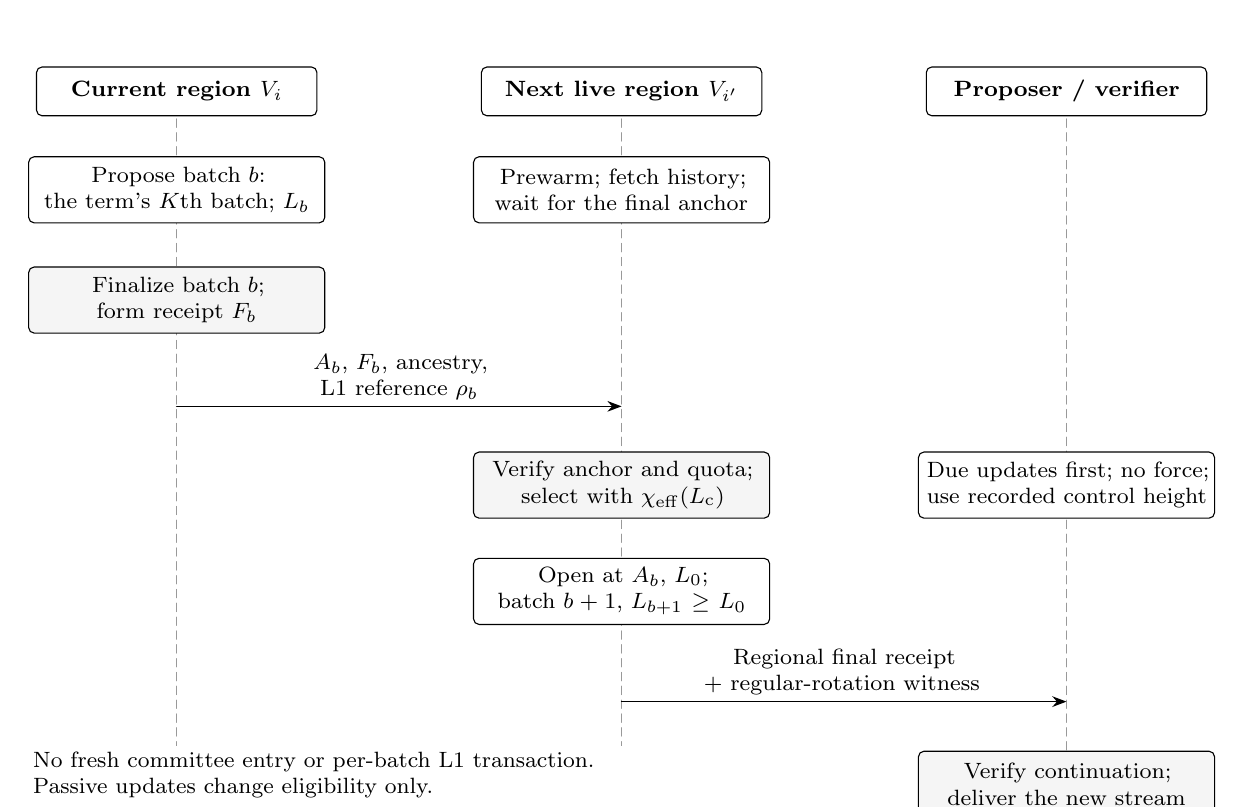
\begin{tikzpicture}[
  x=1cm,y=1cm,font=\footnotesize,line cap=round,line join=round,
  party/.style={draw,rounded corners=2pt,fill=white,align=center,
    text width=3.35cm,minimum height=.62cm,inner sep=3pt},
  action/.style={party,text width=3.55cm,minimum height=.84cm},
  lane/.style={densely dashed,black!40},
  msg/.style={-{Stealth[length=1.8mm]},semithick},
  lab/.style={fill=white,inner sep=2pt,align=center}
]
  \node[party,font=\footnotesize\bfseries] at (2.0,0) {Current region $V_i$};
  \node[party,font=\footnotesize\bfseries] at (7.65,0) {Next live region $V_{i'}$};
  \node[party,font=\footnotesize\bfseries] at (13.3,0) {Proposer / verifier};
  \foreach \x in {2.0,7.65,13.3} \draw[lane] (\x,-.35) -- (\x,-8.72);

  \node[action] at (2.0,-1.25)
    {Propose batch $b$:\\the term's $K$th batch; $L_b$};
  \node[action] at (7.65,-1.25)
    {Prewarm; fetch history;\\wait for the final anchor};
  \node[action,fill=black!4] at (2.0,-2.65)
    {Finalize batch $b$;\\form receipt $F_b$};
  \draw[msg] (2.0,-4.0) -- node[lab,above,text width=4.75cm]
    {$A_b$, $F_b$, ancestry,\\L1 reference $\rho_b$} (7.65,-4.0);
  \node[action,fill=black!4] at (7.65,-5.0)
    {Verify anchor and quota;\\select with $\chi_{\rm eff}(L_{\rm c})$};
  \node[action] at (13.3,-5.0)
    {Due updates first; no force;\\use recorded control height};
  \node[action] at (7.65,-6.35)
    {Open at $A_b$, $L_0$;\\batch $b+1$, $L_{b+1}\geq L_0$};
  \draw[msg] (7.65,-7.75) -- node[lab,above,text width=4.65cm]
    {Regional final receipt\\+ regular-rotation witness} (13.3,-7.75);
  \node[action,fill=black!4] at (13.3,-8.8)
    {Verify continuation;\\deliver the new stream};
  \node[lab,text width=8.6cm,align=left,anchor=west] at (.1,-8.68)
    {No fresh committee entry or per-batch L1 transaction.\\
    Passive updates change eligibility only.};
\end{tikzpicture}

\caption{Regular rotation at quota expiry. Time flows down; spacing is
causal, not to scale. The successor verifies the terminal finalized anchor
and the status map effective at the recorded L1 selection height before
proposing. Passive updates affect
eligibility, not the current term's quota.}
\label{fig:regular}
\end{figure}
\FloatBarrier

\subsection{Forced rotation after active-region failure}\label{sec:forced}
A scheduled map forces rotation only when it becomes effective and leaves
the then-certified active region off. An inactive region's recovery is not
such a trigger. The L1 activation height $a_{j_*}$ specifies when this
obligation arises; it does not specify an application batch.
The recovery witness determines a separate cut $\beta_*$.
Let $\mathcal H$ authenticate the original region/session and prefix.
The operation \Proc{ResolveFinalized} verifies the receipt and ancestry
and returns the anchor at that application height:
\[
 A_{\beta_*}=\Proc{ResolveFinalized}(\beta_*,F_{\beta_*},\mathcal H).
\]
Under regional safety and the accepted authority history, two valid
resolutions at this position have identical application contents.
Different signature encodings do not create a different anchor.

\begin{protocol}{alg:force}{Forced handoff after scheduled activation}
\begin{enumerate}[label=\textbf{F\arabic*.}]
\item \textbf{Trigger.} Advance the control cursor from finalized L1,
independently of APP production. Apply due entries sequentially against
the certified authority state. A passive entry changes eligibility only.
The first entry making the active region off records
$(j_*,a_{j_*},\alpha_*)$; retain this pending handoff even if a later effective map
marks the old region live again. If no force is pending, return. Repeated
observations do not create additional terms.
\item \textbf{Preserve and close.} For the stored trigger and retiring
session, obtain the recovery witness required by \cref{ass:recovery}.
It fixes $\beta_*$ and covers all old finalized work, including work
completed during the notice window or already in flight. Reject a cut
below any retained finalized suffix. Missing evidence or unclosed authority
keeps the wrapper waiting.
\item \textbf{Authenticate.} Verify the announcement and L1 finality through
the activation height, the ordered control history, and the independent
regional receipt, data and ancestry. Resolve $A_{\beta_*}$ at the witness's
application cut. Reconcile the authenticated control cursor with the
anchor's timestamp before selecting a successor. Conflicting valid final evidence is a safety-assumption
failure, not permission for the committee to select a branch.
\item \textbf{Select.} Derive $i'=\Proc{NextLive}(i,\chi)$ from the common
effective map. If no successor exists, retain the pending anchor and
retirement. Use the first admissible subsequent effective control prefix that
enables a successor, then seal that choice. Later passive recovery may
enable this same handoff; it does not create a new failure event or revive
old signing authority.
\item \textbf{Open.} After the update is effective and the closed anchor is
verified, record an opening height $L_0=L_{\rm c}\geq a_{j_*}$, also at
least the anchor's last timestamp. Atomically replace $\alpha$, set $d=0$
and phase active, and clear the
latched pending obligation. Open the new session at $A_{\beta_*}$; start
application batch $\beta_*+1$ with quota $K$. Only the new region signs and finalizes the
new first header and its descendants, with batch timestamps at least
$L_0$ and authority checked at each timestamp.
\item \textbf{Keep the backlog.} Preserve all old application data and
source evidence through the cut. Proposer publication must fill the old
unpublished interval before appending the new region's interval.
\end{enumerate}
\end{protocol}
If the retired session produced no application batch, reuse its authenticated
initial anchor; do not fabricate a receipt for a nonexistent batch.
A finalized announcement does not trigger early replacement. Reaching its
activation height makes the status effective, but does not itself prove
closure or recover missing bytes. Those are separate conditions in F2.
Delayed delivery of an old receipt is checked against its historical
timestamp and the retained cut, rather than discarded merely because L1
has advanced. Recovery time may exceed the notice window.

\smallskip
\Needspace{10\baselineskip}
\noindent\textbf{Example: switching from $A$ to $C$.}
Suppose the region order is $(A,B,C)$, with $A$ active, $B$ off and $C$
live. The committee announces that $A$ will become off at L1 height
$1200$. During the notice window, $A$'s finalized stream advances from
application batch $100$ to $105$.

Once L1 height $1200$ is finalized, the wrapper triggers the handoff.
Suppose recovery proves that batch $105$ is a safe closed cut and retrieves
its data and receipt. The wrapper then skips $B$ and selects $C$.
If the new session opens at control height $1203$, $C$ starts application
batch $106$ with mini-block L1 timestamps at least $1203$ and a fresh quota
$K$. If proposer $P$ has published only through batch $102$, it must publish
old batches $103$--$105$ before appending $C$'s batch $106$.
Thus L1 height $1200$ triggers retirement, while application batch $105$
determines where the new stream continues.

\begin{figure}[H]\centering
% Time flows down. The status certificate authorizes handoff, not a branch hash.
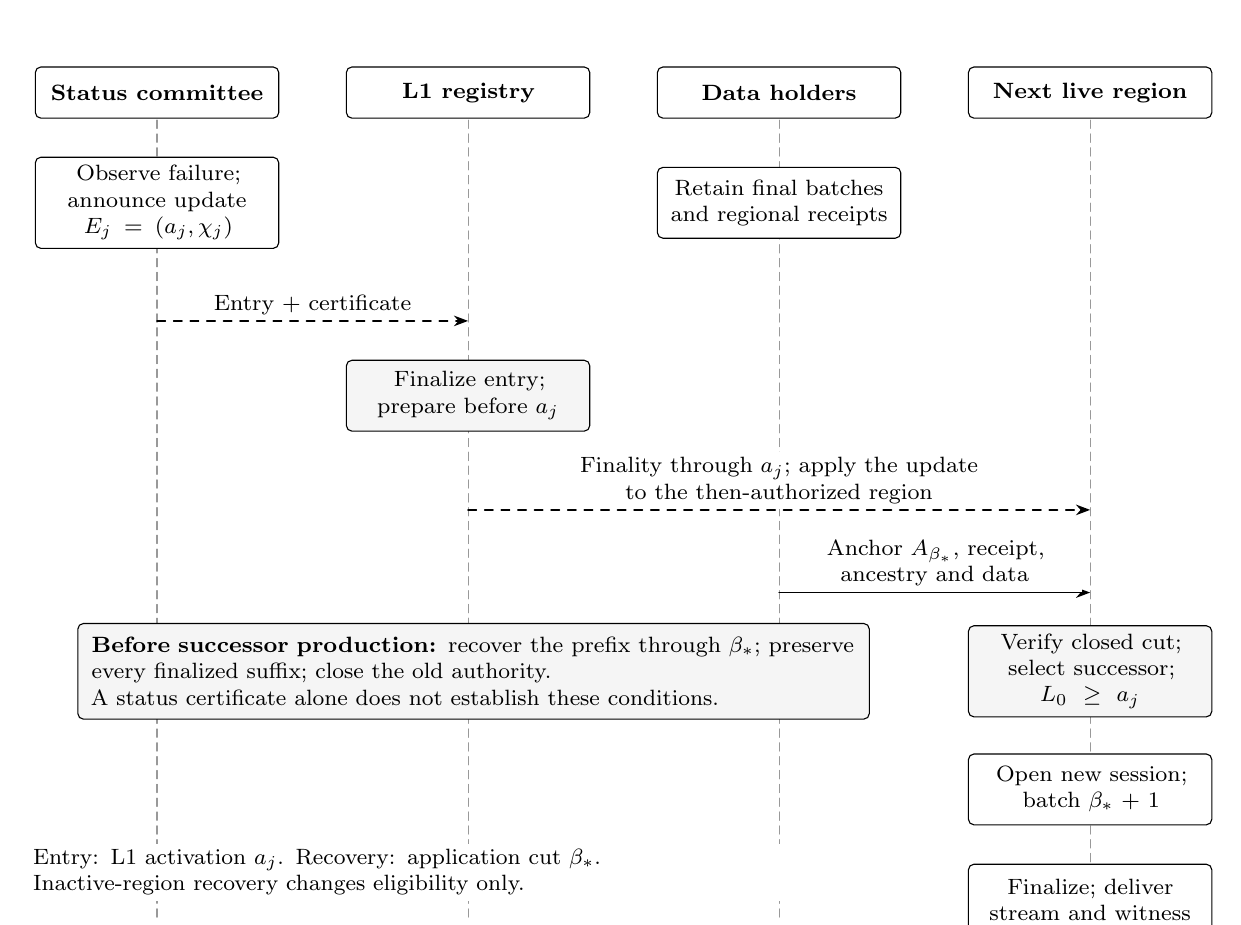
\begin{tikzpicture}[
  x=1cm,y=1cm,font=\footnotesize,line cap=round,line join=round,
  party/.style={draw,rounded corners=2pt,fill=white,align=center,
    text width=2.88cm,minimum height=.65cm,inner sep=3pt},
  action/.style={party,minimum height=.9cm},
  lane/.style={densely dashed,black!40},
  msg/.style={-{Stealth[length=1.8mm]},semithick},
  ctl/.style={msg,dashed},
  lab/.style={fill=white,inner sep=2pt,align=center}
]
  \node[party,font=\footnotesize\bfseries] at (1.7,0) {Status committee};
  \node[party,font=\footnotesize\bfseries] at (5.65,0) {L1 registry};
  \node[party,font=\footnotesize\bfseries] at (9.6,0) {Data holders};
  \node[party,font=\footnotesize\bfseries] at (13.55,0) {Next live region};
  \foreach \x in {1.7,5.65,9.6,13.55} \draw[lane] (\x,-.35) -- (\x,-10.5);

  \node[action] at (1.7,-1.4)
    {Observe failure;\\announce update\\$E_j=(a_j,\chi_j)$};
  \draw[ctl] (1.7,-2.9) -- node[lab,above,text width=3.4cm]
    {Entry + certificate} (5.65,-2.9);
  \node[action,fill=black!4] at (5.65,-3.85)
    {Finalize entry;\\prepare before $a_j$};
  \node[action] at (9.6,-1.4)
    {Retain final batches\\and regional receipts};
  \draw[ctl] (5.65,-5.3) -- node[lab,above,text width=7.2cm]
    {Finality through $a_j$; apply the update\\to the then-authorized region} (13.55,-5.3);
  \draw[msg] (9.6,-6.35) -- node[lab,above,text width=3.6cm]
    {Anchor $A_{\beta_*}$, receipt,\\ancestry and data} (13.55,-6.35);
  \node[action,fill=black!4] at (13.55,-7.35)
    {Verify closed cut;\\select successor;\\$L_0\geq a_j$};
  \node[draw,rounded corners=2pt,fill=black!4,align=left,
    text width=9.7cm,inner sep=5pt] at (5.72,-7.35)
    {\textbf{Before successor production:} recover the prefix through $\beta_*$;
    preserve every finalized suffix; close the old authority.\\
    A status certificate alone does not establish these conditions.};
  \node[action] at (13.55,-8.85)
    {Open new session;\\batch $\beta_*+1$};
  \node[action] at (13.55,-10.25)
    {Finalize; deliver\\stream and witness};
  \node[lab,text width=10.3cm,align=left,anchor=west] at (.05,-9.9)
    {Entry: L1 activation $a_j$. Recovery: application cut $\beta_*$.\\
    Inactive-region recovery changes eligibility only.};
\end{tikzpicture}

\caption{Forced rotation only after the active region becomes unavailable.
The entry schedules an L1 activation height; a separate recovery witness
fixes the application cut. Preparation may start before the status becomes
effective, but a successor starts only after closed-cut and recovery
verification. An inactive region's recovery only changes eligibility.}
\label{fig:forced}
\end{figure}
\FloatBarrier

\subsection{An example and native block boundaries}
Suppose the cyclic list is $(A,B,C)$, region $A$ is active, and $B$ is off.
At ordinary quota expiry, the scheduler selects $C$ if $B$ is still off
at the terminal batch's L1 timestamp. Announcing $B$'s recovery changes
nothing immediately. Once the update is effective, $A$ keeps its session
and remaining quota, while a later eligible handoff may select $B$.
If an update retiring $A$ becomes effective at L1 height $1050$ and
recovery establishes application cut $100$, the successor starts at
application height $101$ with an L1 timestamp at least $1050$.
These two heights have different units. If batch $105$ had already
finalized during preparation, cut $100$ would be invalid.

The abstract service orders mini-block contents. An adapter to a native
format that requires one sequencer key throughout an Ethereum Virtual
Machine (EVM) block must align normal and forced handoff anchors with
complete EVM-block boundaries.
It cannot discard finalized mini-blocks merely to obtain such a boundary.
Batch construction and recovery must make the alignment feasible within
capacity, or the native signing rule must be explicitly extended. Old
mini-blocks retain their original signatures; the new region signs only
its continuation.

\section{Stream Delivery and Rollup Derivation}\label{sec:delivery}
Delivery uses the same interface whether the underlying regional engine is
Sync HotStuff or another SMR. The leader streams mini-block bodies as they
become available and pushes confirmation receipts when ready. Early bodies
can reduce transfer latency, but do not authorize \Tag{Deliver}.
Non-leader replicas retain confirmed data and expose their confirmed frontier,
the last position in their confirmed prefix. The retrieval protocol below
operates within the already derived regional session; cross-region authority
is checked by \Proc{VerifyCross} and the derivation protocol that follows.

\begin{protocol}{alg:retrieval}{Leader stream with peer poll-fetch}
\begin{enumerate}[label=\textbf{D\arabic*.}]
\item \textbf{Push.} Receive the leader's stream of bodies and receipts.
Verify content commitments and buffer objects whose confirmation or predecessor
is missing. Append only a verified contiguous confirmed prefix.
\item \textbf{Poll.} A gap, missing receipt, or periodic poll asks regional
peers for their confirmed frontier. Treat an unsigned tip or bare digest as
a retrieval hint; advancement requires a verifiable receipt.
\item \textbf{Fetch.} Request the missing range and proof from a holder,
trying other configured members after a timeout. Requests and replies have
bounded size; split larger gaps into consecutive ranges.
\item \textbf{Verify and resume.} Check \Proc{VerifyStream}, original producer
authorization, commitments and predecessor continuity. Cache verified objects
and emit each previously undelivered position once. A faulty relay can delay
delivery but cannot change accepted contents.
\end{enumerate}
\end{protocol}

\begin{figure}[H]\centering
% Data availability and transport are separate from the consensus decision.
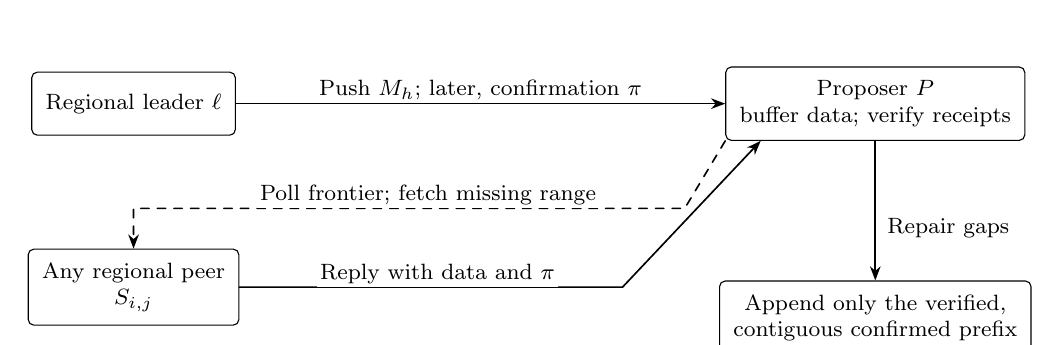
\begin{tikzpicture}[
  x=1cm,y=1cm,font=\footnotesize,line cap=round,line join=round,
  flow/.style={-{Stealth[length=1.8mm]},semithick},
  request/.style={flow,dashed},
  box/.style={draw,rounded corners=2pt,align=center,fill=white,inner sep=5pt},
  lab/.style={fill=white,inner sep=1pt,align=center}
]
  \node[box,minimum width=2.13cm,minimum height=.80cm] (leader) at (1.43,2.80)
    {Regional leader $\ell$};
  \node[box,minimum width=3.78cm,minimum height=.80cm] (proposer) at (10.85,2.80)
    {Proposer $P$\\buffer data; verify receipts};
  \draw[flow] (leader.east) -- node[lab,above] {Push $M_h$; later, confirmation $\pi$} (proposer.west);

  \node[box,minimum width=2.13cm,minimum height=.91cm] (peer) at (1.43,.47)
    {Any regional peer\\$S_{i,j}$};
  \draw[request] (proposer.south west) -- (8.43,1.47) -- (1.43,1.47) -- (peer.north);
  \node[lab,above] at (5.17,1.47) {Poll frontier; fetch missing range};
  \draw[flow] (peer.east) -- (7.64,.47) -- ($(proposer.south west)+(.45,0)$);
  \node[lab,above] at (5.29,.47) {Reply with data and $\pi$};

  \node[box,minimum width=3.78cm,minimum height=.72cm] (deliver) at (10.85,.08)
    {Append only the verified,\\contiguous confirmed prefix};
  \draw[flow] (proposer.south) -- (deliver.north);
  \node[lab,anchor=west] at (10.96,1.22) {Repair gaps};
\end{tikzpicture}

\caption{Push is the primary path; polling and fetching from peers repair
missing data or receipts. All paths pass the same acceptance rule.}
\label{fig:retrieval}
\end{figure}

For the analyzed session, correct replicas retain confirmed bodies and
endorsements and answer bounded requests. A live $P$ eventually reaches such
holders; if no single node has assembled a receipt, $P$ can collect matching
endorsements from them. The model must budget this serving traffic along with
consensus. Recovery from loss of every regional copy, pruning and archive
policy require additional mechanisms. A data-fetch timeout never elects a
leader or grants a different region production authority.

\subsection{Deriving the authorized application history}\label{sec:rollup}
The status registry and the publication frontier are distinct states.
After a forced handoff, the derived control state may already authorize the successor
while publication still owes batches from the old region. Historical
source proofs remain valid through the retained cut; the latest region ID
must not overwrite their authority context.

\begin{protocol}{alg:derive}{Derive and verify the next stream segment}
\textbf{Input:} accepted checkpoint/state $\mathcal Z$, authenticated
registry references, regional batches and transition witnesses.
\begin{enumerate}[label=\textbf{L\arabic*.}]
\item \textbf{Check control history.} Verify canonical L1 block hashes,
finality, registry roots, entry envelopes and ordered control witnesses.
Check the signed batch timestamps, their monotonicity and their complete
registry prefixes. Compute $j(L)$ from activation heights; do not activate
a merely announced entry or omit an intermediate due entry.
\item \textbf{Replay transitions.} Apply effective passive entries without changing
the session or quota. Continue the same region below quota unless a forced
obligation is pending. Apply a latched forced obligation through
\cref{alg:force}; otherwise at quota expiry use \cref{alg:regular}. A local view change uses only
the regional protocol. Replay control advances that occurred without
APP production and process a due update before quota expiry at an equal
control height. Check one immutable successor per sealed boundary and one
accepted recovery cut per retired session.
\item \textbf{Check the regional source.} For each application batch,
derive its region/session and historical member set. Verify its final
receipt, original producer authorization, global batch index, mini-block
range, contents, L1 reference and predecessor. Check equality of the
mini-block references within each batch and the session opening-height
lower bound. Controls contribute no application data.
\item \textbf{Append.} Require a contiguous extension of the accepted
prefix, with each application position processed once. Update the
publication authority cursor along this historical path, including old
backlog before a forced anchor; retain the resulting evidence commitments.
\end{enumerate}
\end{protocol}
A normal rotation needs quota and regional-finality evidence, not a new
committee entry. Conversely, a certificate showing that an inactive region
recovered cannot justify prematurely replacing a healthy active region.
An activation scheduled for L1 height $1050$ cannot be moved by the
proposer, and an accepted application cut cannot be replaced. The verifier
checks old backlog against its historical authority path rather than the
latest effective map.

\subsection{The rollup consistency relation}\label{sec:relation}
Consider a publication covering the inclusive application-batch interval
$[b_-,b_+]$. Let $z_{\rm pre}$ and $z_{\rm post}$ be the execution states
before and after that input. Use $C_{\rm prev}$ for a commitment to the
previously accepted checkpoint and derived authority state,
$C_{\rm in}$ for the complete ordered input, $C_{\rm DA}$ for its DA
encoding, and $C_{\rm registry}$ for the authenticated L1 references used
in the interval. The publication claim is
\[
 y=(\mathit{cfg},C_{\rm prev},[b_-,b_+],C_{\rm in},C_{\rm DA},
       z_{\rm pre},z_{\rm post},C_{\rm registry}),
\]
The witness $w$ contains application batches, regional
receipts, control/snapshot proofs, the transition trace, data and any
execution witness. The rollup consistency relation requires all six
predicates below to hold on this same claim and witness:
\[
 \begin{aligned}
 \mathcal R_{\rm rollup}(y;w)={}&
 \mathcal R_{\rm registry}\land\mathcal R_{\rm source}
 \land\mathcal R_{\rm rotation}\\
 &\land\mathcal R_{\rm input}\land\mathcal R_{\rm DA}
 \land\mathcal R_{\rm exec}.
\end{aligned}
\]
The arguments $(y;w)$ are suppressed on the right-hand side; each
predicate checks the corresponding part of the shared claim and witness.
\begin{description}[style=nextline,leftmargin=1em,labelindent=0pt]
\item[$\mathcal R_{\rm registry}$: authenticated control.]
The entries and timestamped L1 references belong to the stated finalized
history. Domains, signatures, installation lead distances and strictly
increasing activation heights are valid. Complete registry proofs
determine $j(L)$, with future entries pending until due. The witness
preserves the authenticated order of control advances and handoffs.
\item[$\mathcal R_{\rm source}$: regional consensus.]
Each batch's exact contents and ordered mini-block range are covered by a
final receipt from its derived regional session. Historical membership and
original authorship and signed L1 references are correct; a vote QC is not
substituted for a receipt.
\item[$\mathcal R_{\rm rotation}$: authorized succession.]
The claimed state trace satisfies \cref{alg:derive}, including quota,
NextLive, scheduled activation, batch timestamp monotonicity, effective
passive updates, separate forced-cut guards and anchor equality.
Every change of region has the corresponding regular or forced witness.
\item[$\mathcal R_{\rm input}$: faithful ordered data.]
The interval begins immediately after $C_{\rm prev}$, has no omissions or
duplicates, and preserves transaction order, multiplicity, lengths and
mini-block boundaries and signed headers, including their L1 timestamps.
The supplied data opens $C_{\rm in}$; decoding the
data committed by $C_{\rm DA}$ yields exactly the same input. Membership
of a few leaves alone does not prove this complete-range correspondence.
\item[$\mathcal R_{\rm DA}$: availability.]
The chosen DA mechanism's publication, retrievability and retention
conditions hold. A data hash or location string alone is not availability.
\item[$\mathcal R_{\rm exec}$: execution.]
Executing this same ordered input from $z_{\rm pre}$ gives $z_{\rm post}$,
with the required native block rules. Ordering signatures alone do not
establish this equality.
\end{description}

\begin{figure}[htbp]\centering
% Source authorization and execution validity remain distinct proof obligations.
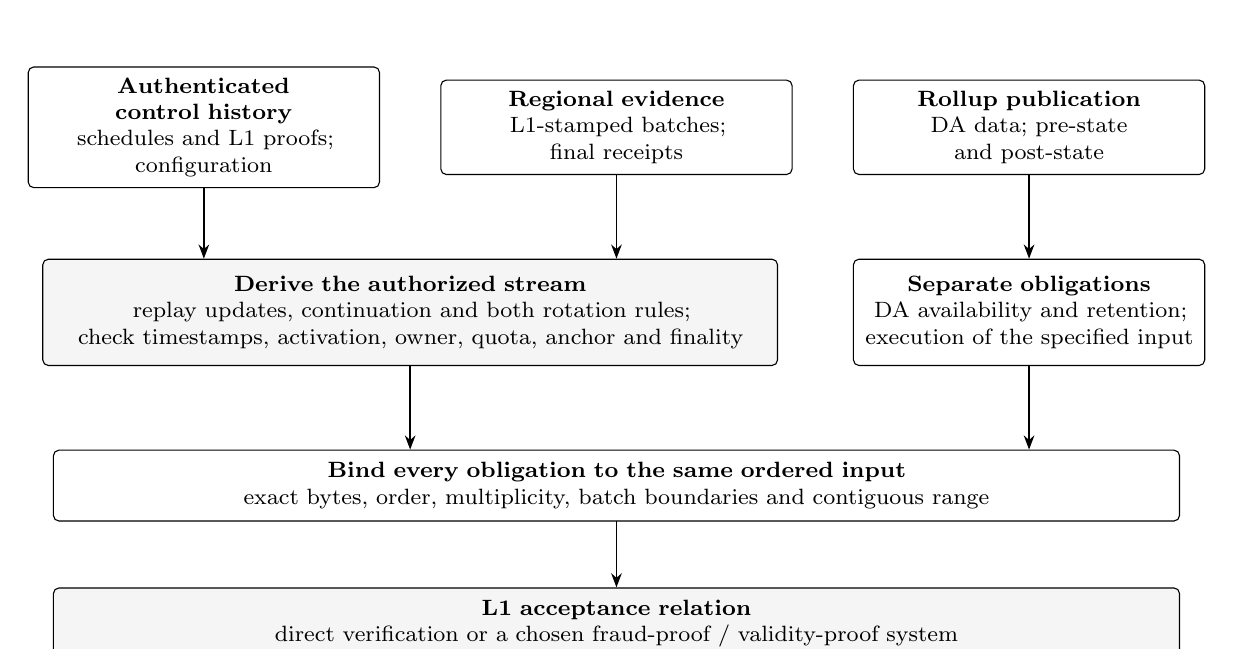
\begin{tikzpicture}[
  x=1cm,y=1cm,font=\footnotesize,line cap=round,line join=round,
  box/.style={draw,rounded corners=2pt,fill=white,align=center,
    inner sep=4pt,minimum height=.85cm},
  flow/.style={-{Stealth[length=1.8mm]},semithick},
  lab/.style={fill=white,inner sep=2pt,align=center}
]
  \node[box,text width=4.18cm] (registry) at (2.38,0)
    {\textbf{Authenticated control history}\\schedules and L1 proofs;\\configuration};
  \node[box,text width=4.18cm] (regional) at (7.62,0)
    {\textbf{Regional evidence}\\L1-stamped batches;\\final receipts};
  \node[box,text width=4.18cm] (published) at (12.86,0)
    {\textbf{Rollup publication}\\DA data; pre-state and post-state};

  \node[box,text width=9.05cm,minimum height=1.35cm,fill=black!4] (derive) at (5.0,-2.35)
    {\textbf{Derive the authorized stream}\\
    replay updates, continuation and both rotation rules;\\
    check timestamps, activation, owner, quota, anchor and finality};
  \draw[flow] (registry.south) -- (registry.south |- derive.north);
  \draw[flow] (regional.south) -- (regional.south |- derive.north);

  \node[box,text width=4.18cm,minimum height=1.35cm] (exec) at (12.86,-2.35)
    {\textbf{Separate obligations}\\DA availability and retention;\\execution of the specified input};
  \draw[flow] (published.south) -- (exec.north);

  \node[box,text width=14.02cm,minimum height=.9cm] (match) at (7.62,-4.55)
    {\textbf{Bind every obligation to the same ordered input}\\
    exact bytes, order, multiplicity, batch boundaries and contiguous range};
  \draw[flow] (derive.south) -- (derive.south |- match.north);
  \draw[flow] (exec.south) -- (exec.south |- match.north);
  \node[box,text width=14.02cm,minimum height=.9cm,fill=black!4] (accept) at (7.62,-6.3)
    {\textbf{L1 acceptance relation}\\
    direct verification or a chosen fraud-proof / validity-proof system};
  \draw[flow] (match.south) -- (accept.north);
\end{tikzpicture}

\caption{Obligations for faithful proposer publication. Status history and
regional evidence determine the authorized ordered stream. Input/DA and
execution checks bind to that same stream. The selected proof system must
cover the whole relation, not only execution.}
\label{fig:derivation}
\end{figure}

\subsection{L1 and proof-system interface}
L1 may verify the relation directly or accept a validity proof for
$\exists w\,\mathcal R_{\rm rollup}(y;w)$. A fraud-proof implementation may
instead record a pending claim and permit challenges to its derivation and
execution trace, with the necessary witnesses available to challengers.
Pending acceptance and completed dispute resolution are different states.
No particular circuit, challenge game or verifier cost is assumed here.

The committee's small entry does not replace regional source evidence.
Prefix receipts, aggregation or recursive proofs may compress that evidence
while preserving the relation. Likewise, a proof system does not derive
\cref{ass:recovery}'s absence of hidden higher final receipts from a low
anchor receipt. That premise belongs to the control/recovery mechanism,
and must be instantiated or retained as an explicit assumption.

\section{Safety, Progress, and Accountability}\label{sec:security}
\subsection{Regional guarantees}
\noindent\textbf{Scope of the inherited arguments.}
The progress argument in this subsection is for the original regional engine
without the tentative quota-triggered BLAME branch in step V1.
\Cref{sec:quota-experiment} explains the resulting proof obligation; none of
\cref{sec:rotation-discussion}'s candidate normal-rotation rules is assumed here.

The following arguments concern one activated stake configuration under
\cref{ass:network}. They specialize the temporal safety argument of
Sync HotStuff~\cite{synchotstuff} to weights and the mini-block application.
Correct nodes preserve votes, committed prefixes and view state across any
permitted restart. L1 references are immutable proposal fields; their
historical validity does not change when a newer L1 block arrives.
Control-triggered retirement must preserve these native rules until a
safe closure boundary under \cref{ass:recovery}; an uncoordinated
per-replica refusal to vote is not covered by the native proof.
Here a \emph{direct commitment} is commitment when a block's own timer
expires. An ancestor may instead be committed when a descendant's timer
expires, as specified in step S4 of \cref{alg:steady}.

\begin{lemma}[Certificate and handover preservation]\label[lemma]{lem:preserve}
If a correct member directly commits $B_k$ in view $v$, no conflicting block
is certified in that view, and every correct member enters view $v+1$ with
an entry lock of rank at least $(v,k)$.
\end{lemma}
\begin{proof}
Suppose the timer expires at time $t$. Its owner forwarded and voted for
$B_k$ at $t-2\Delta_R$, so all correct members receive the proposal by
$t-\Delta_R$. An earlier honest vote for a conflicting proposal would carry
leader-signed conflict evidence back to the timer owner by $t$, forcing it
to quit. A correct member that had already quit by $t-\Delta_R$ would
likewise propagate its quit proof by $t$. Both contradict this commitment.
View-entry skew is at most $\Delta_R$: the first correct quitter relays its
proof, all others quit within one delay, and each then waits one delay.

Thus all correct members can vote for this proposal by $t-\Delta_R$,
without a conflicting vote in that view. Their weight exceeds $2W_i/3$, so
each obtains $Q_v(B_k)$ by $t$. Every vote certificate contains an honest signer;
therefore no conflicting block can certify. The wait before STATUS ensures
a member entering the next view has this certificate or one of higher rank.
\end{proof}

\begin{lemma}[Unique extension across views]\label[lemma]{lem:extension}
After a correct direct commitment of $B$, every certificate of equal or
higher rank identifies $B$ or a descendant.
\end{lemma}
\begin{proof}
The same-view case follows from \cref{lem:preserve} and parent certification.
Suppose the lowest-ranked counterexample in a later view exists. Its quorum
contains an honest voter. If that vote re-certifies a NEWVIEW anchor, the
older certificate selected by NEWVIEW has rank at least the voter's lock,
hence at least the commitment rank, but below the alleged first counterexample.
It would already be a counterexample. If the vote is for a fresh proposal,
its same-view certified parent is a lower-ranked counterexample. Both cases
are impossible. Monotone entry locks preserve the induction.
\end{proof}

\begin{theorem}[SMR and stream safety]\label[theorem]{thm:safety}
Correct replicas have compatible committed block logs. Their command
projections satisfy SMR safety, and correct consumers satisfy the authenticity
and prefix-safety clauses of \cref{def:stream}.
\end{theorem}
\begin{proof}
A direct commitment preserves every earlier direct commitment by
\cref{lem:extension}; committing ancestors preserves the same order.
Hence no position has two committed blocks. Projection fixes both the
batch-command sequence and mini-block sequence. Receipt weight $>W_i/3$
exceeds faulty weight, so each receipt contains an honest post-commit
endorsement. Signature verification and hash
binding fix producer authority, transaction order, L1 references and ancestry, while the
consumer appends only contiguous entries. Retrieval changes the supplier,
not the verified value.
\end{proof}

\begin{theorem}[Progress and delivery]\label[theorem]{thm:progress}
With sufficient service capacity and available L1-reference proofs, a continuously serving regional engine
keeps committing physical blocks. Its finalized application prefixes are
eventually delivered to live consumers. A quota-bounded session that remains
authorized through completion reaches its terminal application receipt.
For an unbounded application service, the input-service clause of
\cref{ass:service} additionally supplies request-level SMR liveness.
\end{theorem}
\begin{proof}
After a quit, entry times differ by at most $\Delta_R$. An honest new leader
waits $2\Delta_R$, so it learns every correct entry lock and selects an anchor
that passes all their rank checks. Re-certification produces its current-view
certificate, after which the leader can propose every $2\Delta_R$ or faster.
Even for the earliest entrant, the first fresh proposal triggers a vote by
$6\Delta_R$ after entry, and the $p$th by $(2p+4)\Delta_R$. Timely arrivals
precede deadline tests, so honest members never blame this leader; faulty
weight alone cannot reach the $>W_i/3$ threshold. Thus no BLAME certificate
can force it to quit, and its proposals commit after their timers.

A Byzantine leader either sustains this proposal progress or causes a quit
through a missed deadline or equivocation. If view changes continue, the
cyclic list reaches an honest leader; if they stop, the continuing
nonconflicting proposal chain commits. The quota adapter counts DRAIN
blocks in native progress tests, so it preserves this argument while
finishing the terminal application ancestor. Retirement ends the old
session's service obligation; it does not promise further application
growth in that session. A prefix committed at only some
members survives handover and, while the engine remains in service, is
committed through a later descendant. At terminal retirement, remaining
consumers can instead learn and deliver the completed application prefix
from its verified final receipt; this is not a new timer-free native commit
rule. Honest members alone can supply the $>W_i/3$ weight required
for BLAME and, after commitment, matching confirmations. Dissemination and
poll-fetch ensure delivery. Finally, a persistently
submitted eligible command selected in an honest-serving interval is included
in a committed batch. This last step uses the stated input-service condition,
not an inferred anti-censorship guarantee.
\end{proof}

Positive conflict evidence attributes incompatible signed statements to a
registered key. This establishes the soundness of the specified evidence
predicates, not a claim that every service failure is slashable. The proof
does not establish safety after the regional synchrony/stake assumptions
fail. The following composition results take regional safety as a premise.

\subsection{Composition across regional sessions}
\begin{lemma}[A fixed anchor determines one normal successor]\label[lemma]{lem:normal}
Under regional safety, the authenticated L1-timestamp rule and the control-order
premise of \cref{ass:recovery}, a sealed normal
handoff has one finalized application anchor and one authorized successor
session, or a fixed pending boundary if no successor is eligible.
\end{lemma}
\begin{proof}
Regional safety fixes the terminal application's contents and ancestry.
Its signed timestamp and complete registry proof fix the initially
effective map. At a waiting boundary, the authenticated control extensions
fix the first admissible completion. The schedule and deterministic list
scan then fix the successor. The session hash binds the resulting term,
region, start height, anchor and opening control height.
No receiver substitutes a later map. A pending boundary consumes its ordered
control extensions until the first admissible completion; it cannot be
completed twice with different successor authority under
\cref{ass:recovery}.
\end{proof}

\begin{theorem}[Cross-region prefix safety]\label[theorem]{thm:cross-safety}
Assume the regional live-stream safety contract for every participating
session, cryptographic validity, \cref{ass:committee,ass:recovery}, and
correct wrapper verification. Then \cref{def:xstream}'s authorized
composition and prefix-safety clauses hold.
\end{theorem}
\begin{proof}
Induct over installed session boundaries from the common initial anchor.
Inside one session, regional safety gives comparable finalized prefixes.
At a normal boundary, \cref{lem:normal} fixes the anchor and successor;
its first batch extends that exact prefix. At a forced boundary, the
recovery cut includes every already accepted or exportable final prefix,
closes competing old authority, and supplies a unique recoverable anchor.
The ordered control rule fixes the due entry and successor, independently
of whether the application stream advances to announce the failure.
Opening-height and monotonicity checks prevent the new continuation from
moving back before its authorizing boundary. Effective passive updates alter
neither current session nor delivered data. Thus every admitted continuation
extends the preceding finalized prefix and no installed authority permits
an incompatible one. Signature/content checks give the claimed sources.
\end{proof}
The theorem is conditional on the recovery cut. A status signature and
L1 finality, signed timestamps and elapsed notice alone do not prove that
premise, nor does labeling a region
unavailable turn a regional synchrony violation into a crash-only fault.

\begin{theorem}[Progress of the composed service]\label[theorem]{thm:cross-progress}
Suppose serving regions satisfy their regional progress and retention
conditions, admitted work fits capacity, and each pending handoff eventually
obtains an admissible cut, an eligible successor and its required data.
Assume committee/L1 and control-delivery progress, finite scheduled
activation waits, available reference proofs, and sufficiently long serving
intervals for new sessions to initialize and finalize application batches.
Then the cross-region stream grows and its confirmed mini-blocks are
eventually delivered to live consumers.
\end{theorem}
\begin{proof}
An available authorized session makes application progress. In a regular
term, the quota adapter supplies physical progress through the terminal
receipt. Finite handoff and successor initialization permit the next term
to serve. If the active region becomes unavailable, L1 and the independent
control cursor eventually reach the scheduled retirement even without new
APPs. The assumed closure and data progress then enable the forced successor. An inactive
recovery alone does not restart a healthy session. The serving-interval
premise excludes an infinite sequence of transitions that never permits
one application batch to finish. Induction yields unbounded application
progress; retained receipts and poll-fetch yield eventual delivery.
\end{proof}
A particular input requires the stated admission and non-starvation policy.
No finite recovery bound follows when all required data are lost, no other
region is eligible, L1 stalls, or a complete safe cut cannot be obtained.

\begin{theorem}[Faithful rollup derivation]\label[theorem]{thm:rollup}
If the verification mechanism soundly enforces $\mathcal R_{\rm rollup}$,
then its accepted completed claims contain the authorized regional-final
input in the specified order and satisfy the stated DA and execution
conditions, under their respective assumptions.
\end{theorem}
\begin{proof}
The registry and rotation predicates fix a legal authority trace and
the scheduled status version at every recorded L1 control height.
The source predicate associates each batch with the regional-final contents
at its position. The input predicate fixes completeness, order and the DA
encoding of those same bytes. The DA and execution predicates supply the
remaining properties. Hence a claim with a substituted region, omitted
input, unrelated DA payload or incorrect execution result fails at least
one conjunct. For a fraud-proof realization, sound enforcement includes
its challenge/availability assumptions and completed dispute procedure;
provisional recording alone is not this conclusion.
\end{proof}

\section{Finality, Throughput, and Communication}\label{sec:complexity}
\subsection{Measurement points and steady-state costs}
Recall that $n_i=|V_i|$ is the regional member count. Let $c$ be the status
committee size and $m=|\mathcal R|$ the number of regions.
A new application batch contains at most $\ell$ body bits;
$\kappa$ bounds the bit length of a signature together with its signer
identifier and a constant number of digests and counters. Certificates below are explicit
signature lists. All message counts mean point-to-point transmissions by
correct participants under the admitted workload; Byzantine wire flooding
is excluded. A batch's mini-block count and body size remain bounded.
The added height and L1 hash fit the bounded header metadata. Let
$s_{\rm ref}$ bound uncached L1 finality and registry evidence carried with
a batch; with a cached reference, this additional payload is zero.

Measure a ready batch's latency from its leader's first proposal transmission.
For an honest, already initialized leader in region $i$, with the required
L1 proofs available and no control-recovery interruption, write
$T_i^{\rm commit}$ for the commitment-latency bound,
$T_i^{\rm receipt}$ for the transferable-receipt bound, and $I_i$ for
the ideal interval between proposals. Then
\[
 \begin{aligned}
 T_i^{\rm commit}&=\delta_R+2\Delta_R,&
 T_i^{\rm receipt}&=T_i^{\rm commit}+\delta_R,&
 I_i&=2\delta_R.
 \end{aligned}
\]
Here $T_i^{\rm commit}$ bounds commitment at every correct regional replica, and $T_i^{\rm receipt}$
is a conservative bound for a transferable final receipt at a regional
collector: after the latest honest commitment, one more regional message
delay collects matching post-commit endorsements. Sending the resulting
complete object to proposer $P$ gives $T_i^{\rm receipt}+\delta_P$. Direct endorsements
to $P$ can avoid this extra collection hop. These expressions presume
that bodies, ancestry and verification fit the stipulated complete-message
bounds; otherwise their additional acquisition time must be added.

The leader can obtain a vote QC and propose the next batch after $I_i$,
while earlier commitment timers continue. Thus $I_i$, not $T_i^{\rm receipt}$, is the
ideal batch interval. Construction time, bandwidth and processing can
increase it. If a batch contains $u$ mini-blocks, $u/I_i$ is its sustained
mini-block rate; it does not imply evenly spaced mini-block finalizations
inside a batch. Transaction throughput additionally depends on batch size.

With full proposal forwarding and unaggregated parent QCs, one regional
physical block costs
\[
 \mathsf{Msgs}_i=O(n_i^2),\qquad
 \mathsf{Bits}_i=O(n_i^2(\ell+s_{\rm ref})+n_i^3\kappa)
\]
messages and bits. Reference-proof fetching and dissemination beyond
these proposals are charged separately; reusing an authenticated origin
does not require a new L1 transaction per batch. The cubic control term arises because an
$O(n_i\kappa)$-bit QC accompanies up to $O(n_i^2)$ forwarded proposals.
Votes and post-commit endorsements contribute $O(n_i^2\kappa)$ additional
bits, already dominated here. Each subscribed external consumer adds
$O(n_i)$ endorsement messages and $O(n_i\kappa)$ control bits per batch;
body retrieval is charged separately. Compact certificates and cached
proposal forwarding may improve these bounds only with their signer,
setup and retrieval costs included.

\subsection{The four operating paths}
In this analysis, $i$ and $j$ identify the source and successor regions.
Let $T_{ij}^{\rm xfer}$ be the complete-object transfer and verification time for an
already assembled anchor receipt and its missing contents to reach the
correct participants of successor region $j$. It includes any necessary
successor-side dissemination; cached contents reduce its payload. Let
$T_j^{\rm init}$ be the time from this common readiness to a current-view certified
anchor. With an honest initial leader, the specified NEWVIEW exchange gives the
conservative good-case bound $T_j^{\rm init}\leq2\Delta_R+2\delta_R$, once the required readiness
skew is satisfied. A separately specified preinitialization mechanism may
reduce $T_j^{\rm init}$; the analysis includes this cost unless such a
mechanism is specified.

Let $T_i^{\rm drain}$ be any terminal-drain delay beyond the steady-state bound $T_i^{\rm receipt}$.
It is zero on the healthy direct-commit path with the terminal registry
proof already available. Recovery of a terminal batch, extra failed leaders,
uncached registry-proof acquisition and missing data are charged separately
or to $T_i^{\rm drain}$; none is hidden in the cached steady-state bound.
Let $T_{ij}^{\rm wait}$ be the additional time spent waiting for an eligible
successor; it is zero when the selected control prefix already supplies one.
For normal rotation define the proposal-to-proposal boundary interval
\[
 H_{ij}=T_i^{\rm receipt}+T_i^{\rm drain}+T_{ij}^{\rm wait}+T_{ij}^{\rm xfer}+T_j^{\rm init}.
\]
It starts when the old region sends its final application-batch proposal
and ends when the new region sends its first fresh proposal. The first
new transferable receipt is available another $T_j^{\rm receipt}$ later.
For local view change, let $T_i^{\rm view}$ be the time from the first
correct quit to the first fresh proposal by an honest next leader, with
the required state already available. For forced rotation, let
$T_{\rm detect}$ be the observation delay, $T_C$ the ordered entry
certification time, and $T_{L1}$ its inclusion and finality wait.
Let $T_{\rm act}$ be the subsequent wait for the scheduled L1 height to
become finalized and for its control proof to reach serving participants.
Let $T_{\rm cut}$ be the residual time after that point for safe-cut
discovery, closure and data recovery, crediting preparation already
completed during the notice window. The following bounds separate these phases:
\[
 \begin{aligned}
 T_i^{\rm view}&=4\Delta_R+2\delta_R,\\
 T_{ij}^{\rm forced}&=T_{\rm detect}+T_C+T_{L1}+T_{\rm act}+T_{\rm cut}\\
                   &\quad+T_{ij}^{\rm wait}+T_{ij}^{\rm xfer}
                         +T_j^{\rm init}+T_j^{\rm receipt}.
 \end{aligned}
\]
The forced-rotation bound ends when the successor's first transferable
receipt is available. It is conditional on each phase completing; the
notice policy does not imply a numerical value of $T_{\rm act}$ without
L1 timing and dissemination bounds. This expression concerns an update
retiring the still-authorized region when it becomes effective.

\begin{table}[H]\centering\small
\begin{tabularx}{\linewidth}{@{}>{\raggedright\arraybackslash}p{.24\linewidth}Y Y@{}}
\toprule
Operating path & Finality or first new final receipt & Batch interval after recovery\\
\midrule
Ideal in-region sequencing & $T_i^{\rm commit}$ to regional commitment;
$T_i^{\rm receipt}$ to a transferable receipt. & $I_i=2\delta_R$.\\
\addlinespace[3pt]
Local view change & From the first correct quit:
$T_i^{\rm view}+T_i^{\rm receipt}$. & $I_i$ after the first fresh proposal.\\
\addlinespace[3pt]
Regular term-end rotation $i\to j$ & From the old terminal proposal:
$H_{ij}+T_j^{\rm receipt}$. From its final receipt: $T_{ij}^{\rm wait}+T_{ij}^{\rm xfer}+T_j^{\rm init}+T_j^{\rm receipt}$. &
$I_j$ within the new term; one boundary interval $H_{ij}$.\\
\addlinespace[3pt]
Forced rotation $i\to j$ & From the outage:
$T_{ij}^{\rm forced}$.
& $I_j$ after recovery; no rate guarantee while waiting for these premises.\\
\bottomrule
\end{tabularx}
\caption{Finality latency and proposal spacing are different metrics.
Add the final consumer-delivery delay to the receipt endpoints.
The forced-rotation expression is a sequential upper bound on the named
phases.}
\label{tab:operating-paths}
\end{table}

The in-region replacement bound follows from the quit protocol. A quit proof
reaches every correct replica within $\Delta_R$; each waits another
$\Delta_R$ before entry; the new leader waits $2\Delta_R$ and then spends
at most $2\delta_R$ re-certifying its anchor. Detection precedes this
measurement. A silent leader's first fresh-proposal deadline is
$6\Delta_R$ after local view entry, but later detection depends on the
deadline index and the attained progress. Additional unsuccessful views
and state transfer are separate costs, not covered by one honest-successor
replacement.

Regular rotation means exhaustion of the fixed quota of $K$ application
batches, not an unsynchronized wall-clock timeout. If a wall-clock tenure
is later added, its authenticated expiry and terminal-cut rules must first
be specified. In a homogeneous fault-free schedule with an available successor
($T_{ij}^{\rm wait}=0$), interval $I$ and boundary interval $H$, the amortized interval and rate are
\[
 \overline I=\frac{(K-1)I+H}{K},
 \qquad \lambda_{\rm batch}=\frac{1}{\overline I}.
\]
The term has $K-1$ internal proposal gaps and one cross-region gap; adding
the new batch's finality latency again would double-count the pipeline.
For heterogeneous regions, average the corresponding sums of internal
gaps and boundary gaps over the actual schedule. Startup and final drain
are boundary effects for a finite measurement window.

The phases of forced rotation may overlap; their sum is a conservative upper
bound, not a tight lower bound. No finite forced-rotation bound
follows without a closed cut, recoverable anchor data, a live successor,
committee progress, L1 activation progress and control delivery. An
effective passive update causes no handoff and does not reset the current
quota; acquiring a new reference proof still incurs its actual cost.

A fault-free term with no discarded or repeated application proposals,
$K$ application blocks and $d_{\rm ctrl}$ physical DRAIN blocks incurs,
before handoff traffic,
\[
 O((K+d_{\rm ctrl})n_i^2)\ \text{messages},\qquad
 O(Kn_i^2(\ell+s_{\rm ref})+(K+d_{\rm ctrl})n_i^3\kappa)\ \text{bits}.
\]
Zero additional drain latency does not mean zero control traffic.
$d_{\rm ctrl}$ is charged explicitly; it is not a protocol-independent
constant. Discarded application attempts, failed views and retrieval add
their actual communication beyond this term bound. At fixed ideal proposal
spacing the control count can scale with
$\Delta_R/\delta_R$, and faults or different admission cadence change it.
Once the terminal receipt closes the physical session, waiting for a
successor creates no further DRAIN proposals; retained-data serving remains.

\subsection{Rotation and registry communication}
One in-region replacement adds $O(n_i^2)$ transmissions and
$O(n_i^3\kappa)$ control bits with explicit certificate lists, plus any
missing ancestral data. NEWVIEW re-certification is included; the first
fresh batch then has the steady-state cost above. If terminal drain emits
$d_{\rm ctrl}$ additional control blocks, charge their proposal and vote exchanges
separately. They consume no application quota and carry no new application
body, although inherited data may still need transfer.

For one normal handoff, suppose one reachable holder already has the
assembled old receipt and sends it to each successor member. Let $a_{ij}$
be the number of missing anchor/ancestry data bits and $s_{L1}$ the size of
the needed registry-history authentication. The outer transfer costs
\[
 O(n_j)\ \text{messages},\qquad
 O\bigl(n_j(a_{ij}+n_i\kappa+s_{L1})\bigr)\ \text{bits}.
\]
Receipt collection has already been charged to the old batch. Successor
bootstrap adds $O(n_j^2)$ messages and $O(n_j^3\kappa)$ control bits with
the specified all-to-all NEWVIEW procedure. Failed retrieval attempts,
additional holders and uncached history add their actual costs. The
$O(n_j)$ outer transfer is not a claim that the regional consensus itself
has linear communication.

A full status map in the fixed region-list order has $O(m)$ bits; an
entry with an explicit committee signature list has size
$s_E=O(m+c\kappa)$. One status update contributes an $O(s_E)$-bit L1
transaction payload; its activation height adds bounded counter metadata.
Disseminating announcement and later activation proofs directly to $N$
interested participants costs $O(N)$ messages and $O(N(s_E+s_{L1}))$ bits. Let $M_C$ and
$B_C$ denote, respectively, the message and bit costs of the committee's
internal observation, agreement and certification. They remain explicit
parameters because threshold
signatures alone do not specify an agreement protocol. A forced
rotation adds these update costs and its data-recovery traffic to the
normal anchor-transfer and successor-bootstrap costs. A passive update
pays registry/control-proof costs and may reduce an already pending
$T_{ij}^{\rm wait}$ only after its activation height is reached.

For comparison, write $M_H,B_H$ for the message and bit costs of a handoff,
and $M_U,B_U$ for those of a status update, including its committee work.
The preceding bounds give
\[
 \begin{aligned}
 M_H&=O(n_j^2),&
 B_H&=O\bigl(n_j(a_{ij}+n_i\kappa+s_{L1})+n_j^3\kappa\bigr),\\
 M_U&=M_C+O(N)+1,&
 B_U&=B_C+O\bigl(s_E+N(s_E+s_{L1})\bigr).
 \end{aligned}
\]
The $1$ in $M_U$ is the registry submission, not Ethereum's internal
consensus traffic. Let $M_{\rm rec},B_{\rm rec}$ count additional cutoff,
fencing and recovery work, excluding transfer already charged in $M_H,B_H$.

\begin{table}[htbp]\centering\small
\begin{tabularx}{\linewidth}{@{}p{.30\linewidth}p{.24\linewidth}Y@{}}
\toprule
Operating path & Messages & Bits\\\midrule
Ideal in-region batch & $O(n_i^2)$ & $O(n_i^2(\ell+s_{\rm ref})+n_i^3\kappa)$\\
One local view change & $O(n_i^2)$ & $O(n_i^3\kappa)$, plus state retrieval\\
Regular cross-region handoff & $M_H$ & $B_H$\\
Forced cross-region handoff & $M_H+M_U+M_{\rm rec}$ & $B_H+B_U+B_{\rm rec}$\\
\bottomrule
\end{tabularx}
\caption{The first row is per application block; the remaining rows are
additional costs per transition, before the new application stream. Charge
failed attempts, terminal DRAIN blocks and additional retrieval separately.
The committee protocol and recovery mechanism determine the parameterized
costs; no linear-consensus claim is implied.}
\label{tab:communication-paths}
\end{table}

\subsection{Rollup verification and storage}
The rollup relation authenticates every included batch, every applicable
scheduled registry update, signed L1 reference and intervening rotation, in addition to data
correspondence, DA and execution. Its direct verification work therefore
depends on the number of batches, regional signatures, status entries and
transaction bytes in the claimed interval. A validity proof or fraud-proof
implementation determines proving, verification, challenge and on-chain
costs; neither constant L1 cost nor a numerical settlement delay follows
from the relation alone. Sequencer finality, transfer to $P$ and L1
settlement are separate endpoints. Retention grows with the confirmed
history unless an independently justified pruning/checkpoint policy is
installed. All timing bounds require enough bandwidth and processing for
the counted messages and bytes. A bounded preparation or recovery time
additionally requires the stated L1 notice and control-delivery conditions;
the regional bound $\Delta_R$ alone does not supply them.

\clearpage
\section{Discussion: Regular Local Rotation and Further Optimization}
\label{sec:rotation-discussion}

This section considers a regular change of leader \emph{inside the same
region}, while retaining BLAME-based recovery for stalled or equivocating
leaders. It does not install a new regional protocol. We distinguish a
conservative extension that completes a fixed application boundary before
handoff, an optional certificate-based opening optimization, and a replacement
of the regional engine by a protocol whose normal pipeline spans leaders.
The last option is how the HotStuff-family implementations examined below
organize ordinary leader progression. Their rules are evidence for design
choices, not proofs for the synchronous engine in this manuscript.

\subsection{Scope of the inherited quota-trigger experiment}
\label{sec:quota-experiment}
The copied Version 3 text of step V1 in \cref{alg:change} includes a tentative
condition that broadcasts BLAME after a predefined proposal count. We retain
that condition as an experiment, but the progress proof in
\cref{thm:progress} applies only to the original missing-progress and
equivocation triggers. In particular, its inference that an honest leader
is never blamed no longer holds under periodic quota-triggered BLAME.
The inherited safety argument relies on proof propagation, stopping old-view
votes, and safe inheritance; it does not require every exit to accuse a
faulty leader. Preserving those steps is therefore a plausible basis for
safety, but does not establish progress under repeated voluntary exits.

Proposal count alone also says nothing about completed timers. For example,
with $\delta_R=0.1$ ms and $\Delta_R=100$ ms, a healthy pipeline can propose
100 batches in approximately 20 ms, before its first $2\Delta_R$ commit
timer expires. An immediate quota-triggered quit can cancel every pending
timer in that view. This is a finite trace showing the missing progress
argument, not a claim of permanent deadlock for every quota interpretation.
If the condition is instead evaluated only at the existing
$(2p+4)\Delta_R$ deadlines, the proposal count may already exceed the
intended quota. A precise extension must specify both what is counted and
when the test is executed.

\subsection{How production HotStuff-family systems advance leaders}
\label{sec:production-rotation}
The sources below were inspected on 29 September 2026. Flow and Aptos code
citations identify repository commits; these are implementation snapshots,
not attestations of the binaries or feature flags used by every mainnet
validator. Official release descriptions are dated separately. In this
subsection $r$ denotes a comparison protocol's round, rather than this
manuscript's long-lived regional view $v$.

\paragraph{Flow: normal QC progression and TC-based recovery.}
Flow's HotStuff implementation describes itself as a Jolteon variant.
Votes for a block in view $r$ are sent to the leader of view $r+1$.
Its pacemaker has separate \texttt{ProcessQC} and \texttt{ProcessTC} paths.
The safety rules accept entry to $r$ directly when the parent QC has view
$r-1$; otherwise they require the preceding view's TC and check the QC
against the TC's newest QC. A local timeout alone does not advance the
view. Normal rotation consequently needs no timeout accusation, while
failed views have an explicit recovery certificate~\cite{flowcode}.
The finalization layer uses a certified child in the immediately following
view to finalize its parent. Progression and finalization are distinct
tests; a single parent QC is not interchangeable with the receipt of
\cref{sec:receipt}. Flow's engineering account explains that its active
pacemaker and shorter finalization rule were introduced together~\cite{flowjolteon}.

\paragraph{Aptos: the distinction is explicit in the round state.}
At commit \texttt{a19dae54b565}, \texttt{RoundState::process\_certificates}
sets the next round from the highest certificate and records its reason as
\texttt{QCReady} or \texttt{Timeout}. The inspected ordinary voting path
sends votes to the next round's elected proposer unless vote broadcasting
is configured. The same source also contains optimistic proposal handling:
when materializing an optimistic proposal, it checks both the parent QC's
round and the parent's identity. We therefore describe this as evidence
for certificate-driven progression, not as an exhaustive account of all
configured execution paths~\cite{aptosround,aptosmanager}.
The official 20 June 2025 Baby Raptr announcement describes an upgrade to
the Jolteon* and Quorum Store pipeline, including retrieval and verification
of batch contents before voting~\cite{aptosbaby}. An older DiemBFT account
alone is insufficient to characterize the current implementation. The
relevant lesson is that proposer selection, certified round advancement,
data readiness, and final commitment remain separate responsibilities.

\paragraph{Monad: next-leader collection also needs a recovery design.}
MonadBFT's documented normal path sends votes to the next scheduled leader,
which assembles the parent QC and proposes its child. Later certified
extensions finalize earlier blocks; speculative and full finality are
distinguished~\cite{monaddocs}. Its 21 November 2025 recovery update describes
backup votes sent to the current leader as well as the next leader, backup
QC dissemination, and votes carried in timeout messages that may reconstruct
a missing QC. More difficult cases retain reproposal and no-endorsement
certificates~\cite{monadrecovery}. These mechanisms address a specific risk:
a successor can withhold the votes it collects and attempt to discard its
predecessor's unfinalized tail. The current MonadBFT paper treats this
tail-forking resistance as a property beyond ordinary finalized-prefix
safety~\cite{monadpaper}. A transplant of next-leader vote routing without
the corresponding recovery rules would omit the main issue at the boundary.

\begin{table}[htbp]\centering\small
\begin{tabularx}{\linewidth}{@{}>{\raggedright\arraybackslash}p{.17\linewidth}Y Y@{}}\toprule
System & Ordinary advancement & Failure path and lesson\\\midrule
Flow & Parent QC enables the following view and its leader. & TC proves a skipped
view; voting rules constrain which certified parent may be extended.\\
Aptos snapshot & Explicit QC-ready versus timeout-driven round events. & Recovery
and optimistic proposal handling retain certificate checks and data prerequisites.\\
MonadBFT & Next leader collects votes and carries the resulting QC forward. &
Backup collection, timeout evidence and reproposal rules protect supported tails.\\
Current regional engine & QC enables another proposal by the \emph{same}
leader; timers establish commitment. & BLAME/equivocation exits the view;
STATUS and NEWVIEW recover a safe anchor.\\\bottomrule
\end{tabularx}
\caption{The transferable distinction is successful advancement versus failure
recovery. The commit rules, certificate meanings and fault assumptions are
specific to each engine.}
\label{tab:real-world-rotation}
\end{table}

An ordinary proposal-chain sketch is
\[
 L_r:B_k\ \longrightarrow\ \text{votes collected by }L_{r+1}
 \ \longrightarrow\ L_{r+1}:(B_{k+1},Q_r(B_k)).
\]
Neither the arrow nor the QC asserts that $B_k$ is already final. Replacing
the current engine with a chained protocol requires adopting its compatible
locking, commit and timeout rules together. Jolteon's two-chain construction
and its recovery predicates are developed as one protocol~\cite{jolteon}.

\subsection{Candidate A: complete a fixed boundary before normal handoff}
\label{sec:local-boundary-design}
Introduce a local segment index $e$ and a per-segment application quota
$K_{\rm loc}\geq1$, distinct from the cross-region quota $K$. A segment may
contain several recovery views $v$. If its first application height is
$b_e$ and the current term's last allowed height is $b_{\rm term}$, define
\[
 \bar b_e=\min\{b_e+K_{\rm loc}-1,b_{\rm term}\},\qquad
 q_e=\bar b_e-b_e+1.
\]
These quantities are derived from the authenticated opening state. Every
recovery view of segment $e$ retains the same endpoint $\bar b_e$.
Normal completion moves to $(e+1,0)$; a failure moves to $(e,v+1)$.
For example, the scheduled leader could be
\[
 \ell_i(e,v)=\mathcal L_i[(e+v)\bmod n_i].
\]
This is a candidate scheduling rule. After recovery, the next segment's
scheduled leader can coincide with the last recovery leader; a requirement
to exclude that identity would need a different authenticated schedule.

\begin{mdframed}[linewidth=.6pt,skipabove=9pt,skipbelow=9pt]
\small\noindent\textbf{Design sketch A: final-boundary local rotation.}
\begin{enumerate}[label=\textbf{A\arabic*.}]
\item \textbf{Bound admission.} Validate the complete proposed ancestry and
reject an APP beyond $\bar b_e$ in this segment, including attempts in a later
recovery view. The local counter does not reset on failure.
\item \textbf{Finish.} After the terminal APP is proposed, preserve its
commit timer. Fresh descendants may be DRAIN blocks, following the existing
completion adapter. Reaching the quota emits no BLAME and cancels no timer.
\item \textbf{Recover if necessary.} A genuine progress failure or
equivocation invokes the existing recovery path within segment $e$.
If NEWVIEW inherits the terminal APP without a running timer, a fresh DRAIN
descendant can complete it. The remaining application quota stays zero.
\item \textbf{Export a final boundary.} Any holder may disseminate the
terminal receipt $F_{\bar b_e}$, anchor $A_{\bar b_e}$ and missing data.
Completion does not require a release signature from the old leader.
\item \textbf{Open the successor segment.} Provided the region is still
authorized and the cross-region term has not ended, use the verified anchor
as the next segment's initial checkpoint. Conservatively retain the existing
NEWVIEW initialization. The first fresh APP has height $\bar b_e+1$.
\end{enumerate}
\end{mdframed}

The conservative realization treats each segment as a separately named
internal SMR instance, for example with instance identifier
$s_e=\Hash(\Tag{SEGMENT},s,e,A_{b_e-1})$. Its signing and timer contexts
include this identifier. A normal opening initializes the next instance
from a final checkpoint; it is not a timer-free direct commit inside the
old instance. Global application and mini-block heights, regional authority,
the outer term counter and its remaining quota continue unchanged.

This separation matters for DRAIN. The old physical log may extend beyond
the terminal application block through control-only descendants. Those
records are retained in the old instance; the new instance's root represents
the finalized application checkpoint. The proposed composition promises
continuity of the application projection. It does not silently discard
committed physical entries from a single continuing SMR log. A design that
instead retains one physical log must specify and certify its physical
terminal anchor as well.

The hard endpoint and the final receipt do different work. The endpoint
excludes every old-segment APP beyond $\bar b_e$; the receipt fixes the
contents through that endpoint. A receipt for a merely local ``latest
block'', without a common endpoint, supplies no closure guarantee.
Normal closure, delayed old-view recovery, and acceptance of the new
instance still require the composition argument listed below.

\subsection{Candidate A+: replace initialization with an explicit opening certificate}
\label{sec:ready-open-design}
Once the terminal anchor is final, the original leader need not release the
segment and a new leader need not discover an unknown highest old-view
anchor. An optional optimization is to make installation of the common
checkpoint explicit. Define the candidate boundary statement and evidence
\[
 \begin{aligned}
 R_e&=(\mathit{cfg},s,e,e+1,\bar b_e,A_{\bar b_e},\ell_i(e+1,0)),\\
 \mathcal H_e&=(R_e,F_{\bar b_e},\text{required ancestry and authority evidence}).
 \end{aligned}
\]
The hashed statement uses canonical block identities, not the encoding of
a particular signature list. Thus two encodings of the same final receipt
cannot create competing checkpoint identities.

After validating $\mathcal H_e$ and acquiring the data, a member may persist
the next instance's root and sign
\[
 \Sig_S(\Tag{READY},s,e+1,\Hash(R_e)).
\]
READY messages are disseminated so a failed collector cannot permanently
withhold the opening evidence. A candidate opening certificate $O_{e+1}$
contains matching READY signatures of weight $>2W_i/3$. Signers endorse at
most one root for this next-instance identifier, with that state durable
before sending. The next leader's first proposal carries $O_{e+1}$ and
extends exactly the installed anchor.

This is a \emph{new initialization rule}, not an ordinary old-view vote QC.
The first-proposal predicate must explicitly accept the opening certificate;
subsequent proposals return to the chosen engine's normal parent-QC rule.
The existing $>W_i/3$ final receipt establishes past commitment, whereas
the proposed $>2W_i/3$ READY set attests to checkpoint installation. Neither
threshold can be substituted for the other merely because both objects are
called certificates. READY also cannot prove closure of an unrestricted old
stream; the fixed boundary and its finality are prerequisites.

Before any opening certificate exists, missing terminal evidence keeps the
old segment in completion/recovery. After a valid opening is disseminated,
failure of its scheduled leader must enter recovery in the new instance at
the same installed root. Entry skew, timeout start points, certificate
availability, and the race between these cases remain explicit design
obligations. Merely collecting READY signatures is not a complete pacemaker.

\begin{figure}[htbp]\centering
% Discussion sketches; causal ordering only, not a time scale.
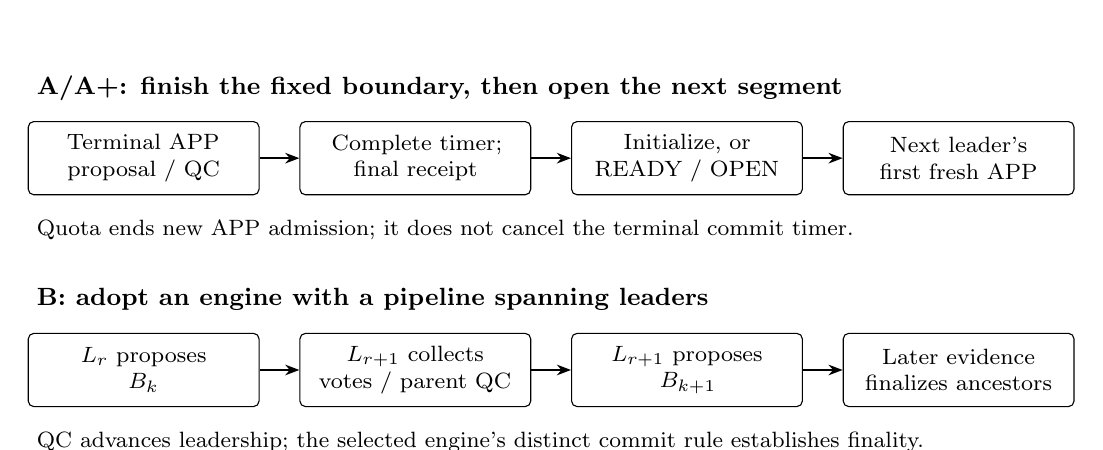
\begin{tikzpicture}[
  x=1cm,y=1cm,font=\footnotesize,
  box/.style={draw,rounded corners=2pt,align=center,text width=2.65cm,
              minimum height=.93cm,inner sep=4pt},
  flow/.style={-{Stealth[length=1.8mm]},semithick}
]
\node[anchor=west,font=\small\bfseries] at (-1.48,2.03)
  {A/A+: finish the fixed boundary, then open the next segment};
\node[box] (a) at (0,1.14) {Terminal APP\\proposal / QC};
\node[box] (b) at (3.45,1.14) {Complete timer;\\final receipt};
\node[box] (c) at (6.9,1.14) {Initialize, or\\READY / OPEN};
\node[box] (d) at (10.35,1.14) {Next leader's\\first fresh APP};
\draw[flow] (a)--(b); \draw[flow] (b)--(c); \draw[flow] (c)--(d);
\node[anchor=west,align=left] at (-1.48,.23)
  {Quota ends new APP admission; it does not cancel the terminal commit timer.};

\node[anchor=west,font=\small\bfseries] at (-1.48,-.65)
  {B: adopt an engine with a pipeline spanning leaders};
\node[box] (e) at (0,-1.55) {$L_r$ proposes\\$B_k$};
\node[box] (f) at (3.45,-1.55) {$L_{r+1}$ collects\\votes / parent QC};
\node[box] (g) at (6.9,-1.55) {$L_{r+1}$ proposes\\$B_{k+1}$};
\node[box] (h) at (10.35,-1.55) {Later evidence\\finalizes ancestors};
\draw[flow] (e)--(f); \draw[flow] (f)--(g); \draw[flow] (g)--(h);
\node[anchor=west,align=left] at (-1.48,-2.46)
  {QC advances leadership; the selected engine's distinct commit rule establishes finality.};
\end{tikzpicture}

\caption{Two optimization levels. Candidate A/A+ waits for the fixed terminal
application receipt; A+ changes only the subsequent opening procedure.
Candidate B permits normal leader advancement before finality by adopting
a compatible consensus engine. Arrows show causal dependencies, not timing
to scale. These are discussion sketches, not additional established protocols.}
\label{fig:local-rotation-options}
\end{figure}

\subsection{Candidate B: a pipeline whose normal progression crosses leaders}
\label{sec:qc-rotation-design}
If waiting for terminal finality at every local boundary is too expensive,
the more substantial optimization is a regional engine with QC-driven
normal leader progression, as in the implementations above. A certified
parent can then enable the next scheduled leader while an earlier block is
still progressing toward the engine's finality condition. The engine's
final output, rather than a bare vote QC, must feed the existing stream
receipt and proposer interfaces.

This cannot be implemented in the present synchronous engine by merely
changing the leader after each QC. Step S4 requires a timer to expire while
the member is still in its view, and S1 requires a current-view parent QC.
The preservation proof also uses quit propagation and the wait before the
next entry lock. A direct cross-leader QC transition changes all three
dependencies. Carrying an old timer across such a transition without a new
proof is equally unsupported.

There are two possible research routes. One is to adopt a particular
partially synchronous chained HotStuff-family engine and prove that its
finality/export interface implements the regional service. The other is
to keep synchronous finality while adopting a purpose-built rotating-leader
construction. Abraham, Nayak and Shrestha give a synchronous construction
with responsive proposal progression across leaders and $2\Delta+O(\delta)$
good-case commitment latency~\cite{rotatingsync}. Its epoch synchronization,
certificate handling and commit timers are part of that construction.
Its count-based assumptions and its lower bound for
$n/3\leq f<n/2$ do not directly establish a lower bound or an upper bound
for this manuscript's stake-weighted, below-one-third model.

Next-leader vote collection can reduce ordinary message fanout, but makes
QC availability at a faulty successor a design concern. Backup collection
and reconstruction from retained votes are relevant optimizations to study.
The present all-to-all regional votes already disseminate this information;
removing that dissemination changes both communication and recovery.
Similarly, aggregate signatures can reduce repeated certificate payloads,
but signer identification, voting-weight checks, setup and retrieval costs
must remain in the analysis. None of these changes is included in the
baseline costs of \cref{sec:complexity}.

\subsection{Timing and communication to measure for the candidates}
Let $T_{i,e}^{\rm boundary}$ run from the terminal APP proposal until its
final receipt is assembled. It equals the baseline $T_i^{\rm receipt}$ on
the healthy direct-commit path, with additional completion/recovery costs
otherwise. Let $T_{i,e}^{\rm local\text{-}xfer}$ include remaining receipt/data
dissemination and readiness at the same regional membership. It must not
be set to zero just because the membership is unchanged. For Candidate A,
the terminal-to-next-proposal interval is
\[
 H_{i,e}^{A}=T_{i,e}^{\rm boundary}
            +T_{i,e}^{\rm local\text{-}xfer}+T_{i,e+1}^{\rm init},
 \qquad T_{i,e+1}^{\rm init}\leq2\Delta_R+2\delta_R
\]
under the baseline honest-leader initialization and readiness premises.
For Candidate A+, define $T_{i,e}^{\rm open}$ from the same assembled-receipt
endpoint through dissemination, READY collection, opening and the first
new proposal. Then
\[
 H_{i,e}^{A+}=T_{i,e}^{\rm boundary}+T_{i,e}^{\rm open}.
\]
With cached data, an honest successor and a fully specified opening
pacemaker, $T_{i,e}^{\rm open}=O(\delta_R)$ is a design target. It is not a
proved bound in this version, and it does not remove the preceding
$2\Delta_R$ terminal commitment wait.

For homogeneous fault-free segments of $q$ APP batches, with no outer-term
boundary in the measurement window, the same proposal-gap accounting gives
\[
 \bar I_{\rm loc}=\frac{(q-1)I_i+H_{\rm loc}}{q},\qquad
 \lambda_{\rm loc}=\frac{q}{(q-1)I_i+H_{\rm loc}}.
\]
For a finite outer term, sum its actual internal, local-boundary and
cross-region gaps. A coincident local and cross-region endpoint has one
successor opening, not two sequential handoffs. Failed attempts and all
DRAIN blocks retain their actual costs.

Candidate A pays the already analyzed initialization exchanges for every
local segment. In A+, all-to-all READY dissemination takes $O(n_i^2)$
messages. With cached boundary evidence, its short signatures alone cost
$O(n_i^2\kappa)$ bits; repeatedly attaching or forwarding explicit
$O(n_i\kappa)$-bit certificates can restore an $O(n_i^3\kappa)$ control
term. Missing data is additional. Therefore a shorter opening delay does
not automatically imply linear communication. Candidate B requires fresh
accounting from the selected engine, including its failure path and the
post-finality receipt exports used here.

\subsection{Proof obligations and evaluation priorities}
\label{sec:rotation-obligations}
Before any candidate becomes normative, it must discharge the following
obligations rather than inherit them from its name or from an implementation
with different assumptions.
\begin{enumerate}[label=\textbf{P\arabic*.}]
\item \textbf{Unique boundary and successor.} Every accepted terminal
receipt for segment $e$ determines the same application anchor; normal
opening and delayed recovery cannot authorize competing successors or
application positions. The claim includes the physical-log/application
projection distinction.
\item \textbf{Preservation under overlap.} A node learning a terminal
receipt while peers are recovering cannot cause loss of completed honest
work. READY persistence, late votes, timer retirement and data retention
must be reconciled explicitly. Old release signatures are unnecessary.
\item \textbf{Completion before normal advancement.} For A/A+, quota
completion keeps pending timers alive and recovery does not repeatedly
reset the segment. Establish eventual terminal finality and opening even
if the scheduled successor or a collector fails. For B, establish the
corresponding chain-based progress property instead.
\item \textbf{Leader schedule compatible with weights.} Faulty stake below
$W_i/3$ does not imply that fewer than one third of identities are faulty.
For example, one honest identity may hold $0.8W_i$ and three faulty identities
the remaining $0.2W_i$. A once-per-identity cycle then has no consecutive
honest leaders. A chained engine whose progress argument needs such a run
cannot infer it from the current assumptions. Its schedule, leader tenure
or probabilistic progress premise must supply what its proof requires.
\item \textbf{Outer authority and consumer compatibility.} A local opening
does not reset $K$, bypass an effective L1 retirement or alter delivered
prefixes. The rollup verifier must authenticate local-segment succession if
it becomes part of signing authority. Execution, DA and L1 settlement keep
their separate meanings.
\item \textbf{Measured endpoints.} Measure proposal spacing, terminal
finality, first successor receipt, recovery delay and bytes separately.
Include $K_{\rm loc}=1$, small $\delta_R/\Delta_R$, missing ancestry, a
withholding QC collector, overlapping receipt and timeout delivery, and
coincident local/outer/L1 boundaries. A bounded simulation can expose bad
traces but does not replace the weighted safety and progress proofs.
\end{enumerate}

The immediate extension to formalize is Candidate A: fixed application
segments, final-boundary completion and ordinary initialization, with
BLAME reserved for recovery. A+ isolates a subsequent startup optimization.
Candidate B addresses the stronger goal of sustaining a pipeline across
leaders without draining it at every normal boundary; it is an engine
change and should receive its own specification and proof before replacing
the regional baseline.


\begin{thebibliography}{99}\small
\setlength{\itemsep}{3pt}
\bibitem{synchotstuff}
I. Abraham, D. Malkhi, K. Nayak, L. Ren, and M. Yin.
\emph{Sync HotStuff: Simple and Practical Synchronous State Machine Replication}.
IEEE Symposium on Security and Privacy, 2020.
This draft uses the 4 May 2020 ePrint revision, Section II, Figures 1--2.
\url{https://eprint.iacr.org/2019/270}.
\bibitem{schneider}
F. B. Schneider.
\emph{Implementing Fault-Tolerant Services Using the State Machine Approach:
A Tutorial}. ACM Computing Surveys 22(4), 299--319, 1990.
\url{https://www.cs.cornell.edu/fbs/publications/SMSurvey.pdf}.
\bibitem{poscompiler}
J. Komatovic, A. Lewis-Pye, J. Neu, T. Roughgarden, and E. N. Tas.
\emph{From Permissioned to Proof-of-Stake Consensus}.
AFT 2025, LIPIcs 354, 18:1--18:26.
\url{https://doi.org/10.4230/LIPIcs.AFT.2025.18}.

\bibitem{flowcode}
Flow contributors. \emph{Flow Go: HotStuff consensus implementation}.
Commit \texttt{4315a94dce27} (25 September 2026).
\href{https://github.com/onflow/flow-go/blob/4315a94dce27b0a5da53103bd1f1f519ba4506ca/consensus/hotstuff/README.md}{Consensus overview};
\href{https://github.com/onflow/flow-go/blob/4315a94dce27b0a5da53103bd1f1f519ba4506ca/consensus/hotstuff/pacemaker/pacemaker.go}{pacemaker};
\href{https://github.com/onflow/flow-go/blob/4315a94dce27b0a5da53103bd1f1f519ba4506ca/consensus/hotstuff/safetyrules/safety_rules.go}{safety rules}.
\bibitem{flowjolteon}
Flow Engineering. \emph{Jolteon: Advancing Flow's consensus algorithm}.
\href{https://flow.com/engineering-blogs/jolteon-advancing-flows-consensus-algorithm}{Official engineering article}. Accessed 29 September 2026.
\bibitem{aptosround}
Aptos contributors. \emph{Aptos Core: round state}.
Commit \texttt{a19dae54b565} (29 September 2026),
\href{https://github.com/aptos-labs/aptos-core/blob/a19dae54b5657cdf7abbd9907f465553cdff07f4/consensus/src/liveness/round_state.rs#L245-L288}{\texttt{process\_certificates}}.
\bibitem{aptosmanager}
Aptos contributors. \emph{Aptos Core: round manager}.
Same commit as~\cite{aptosround}.
\href{https://github.com/aptos-labs/aptos-core/blob/a19dae54b5657cdf7abbd9907f465553cdff07f4/consensus/src/round_manager.rs#L1551-L1573}{Vote routing};
\href{https://github.com/aptos-labs/aptos-core/blob/a19dae54b5657cdf7abbd9907f465553cdff07f4/consensus/src/round_manager.rs#L965-L986}{optimistic proposal materialization}.
\bibitem{aptosbaby}
Aptos Foundation. \emph{Baby Raptr Is Here: a New Era of Consensus Begins}.
20 June 2025.
\href{https://aptosnetwork.com/currents/baby-raptr-lands-on-mainnet}{Official deployment announcement}.
\bibitem{monaddocs}
Monad. \emph{MonadBFT}. Developer documentation.
\href{https://docs.monad.xyz/monad-arch/consensus/monad-bft}{Normal path, finality and recovery}. Accessed 29 September 2026.
\bibitem{monadrecovery}
Category Labs. \emph{MonadBFT Update: Fast Recovery \& Leader Fault Isolation}.
21 November 2025.
\href{https://www.category.xyz/blogs/monadbft-update-fast-recovery-leader-fault-isolation}{Official protocol update}.
\bibitem{monadpaper}
M. M. Jalalzai et al.
\emph{MonadBFT: Fast, Responsive, Fork-Resistant Streamlined Consensus}.
\href{https://arxiv.org/abs/2502.20692v4}{arXiv:2502.20692v4}, 21 July 2026.
\bibitem{jolteon}
R. Gelashvili, L. Kokoris-Kogias, A. Sonnino, A. Spiegelman, and Z. Xiang.
\emph{Jolteon and Ditto: Network-Adaptive Efficient Consensus with Asynchronous Fallback}.
\href{https://arxiv.org/abs/2106.10362v3}{arXiv:2106.10362v3}.
\bibitem{rotatingsync}
I. Abraham, K. Nayak, and N. Shrestha.
\emph{Optimal Good-Case Latency for Rotating Leader Synchronous BFT}.
OPODIS 2021, LIPIcs 217, 27:1--27:19.
\href{https://doi.org/10.4230/LIPIcs.OPODIS.2021.27}{Published article}.
\end{thebibliography}
\end{document}
